\documentclass[12pt,a4paper,twoside,openright]{report}
\usepackage[pdfborder={0 0 0}]{hyperref}    % turns references into hyperlinks
\usepackage[margin=25mm]{geometry}  % adjusts page layout
\usepackage{graphicx}  % allows inclusion of PDF, PNG and JPG images
\usepackage{verbatim}
\usepackage{docmute}   % only needed to allow inclusion of proposal.tex
\usepackage[noend]{algpseudocode}
\usepackage[]{algorithm}
\usepackage{amsmath}
\usepackage{mathtools}
\usepackage{enumitem}
\usepackage{epstopdf}
\newcommand{\var}[1]{{\operatorname{\mathit{#1}}}}

\raggedbottom                           % try to avoid widows and orphans
\sloppy
\clubpenalty1000%
\widowpenalty1000%

\renewcommand{\baselinestretch}{1.1}    % adjust line spacing to make
                                        % more readable

\begin{document}

\bibliographystyle{plain}


%%%%%%%%%%%%%%%%%%%%%%%%%%%%%%%%%%%%%%%%%%%%%%%%%%%%%%%%%%%%%%%%%%%%%%%%
% Title


\pagestyle{empty}

\rightline{\LARGE \textbf{Artjoms Iskovs}}

\vspace*{60mm}
\begin{center}
\Huge
\textbf{Predicting drug-pathway interactions using the Correlated Topic Model} \\[5mm]
Computer Science Tripos -- Part II \\[5mm]
Trinity College \\[5mm]
\today  % today's date
\end{center}

%%%%%%%%%%%%%%%%%%%%%%%%%%%%%%%%%%%%%%%%%%%%%%%%%%%%%%%%%%%%%%%%%%%%%%%%%%%%%%
% Proforma, table of contents and list of figures

\pagestyle{plain}

\chapter*{Proforma}

{\large
\begin{tabular}{ll}
Name:               & \bf Artjoms Iskovs                       \\
College:            & \bf Trinity College                     \\
Project Title:     & \bf Predicting drug-pathway interactions using the Correlated Topic Model\\
Examination:        & \bf Computer Science Tripos -- Part II, July 2015  \\
Word Count:         & \bf ??\\
Project Originator: & N.~Pratanwanich                    \\
Supervisor:         & N.~Pratanwanich                    \\ 
\end{tabular}
}

\section*{Original Aims of the Project}
Implement the Correlated Topic Model for the problem of inferring pathways from drug gene expression data. Find a way to enforce gene-pathway membership priors so that the recovered topic structure can be related to the real data.

\section*{Work Completed}

\section*{Special Difficulties}
None
 
\newpage
\section*{Declaration}

I, Artjoms Iskovs of Trinity College, being a candidate for Part II of the Computer
Science Tripos, hereby declare that this dissertation and the work described in it are my own work,
unaided except as may be specified below, and that the dissertation does not contain material that has already been used to any substantial
extent for a comparable purpose.

\bigskip
\leftline{Signed [signature]}

\medskip
\leftline{Date [date]}

\tableofcontents

\listoffigures

\newpage
\section*{Acknowledgements}


%%%%%%%%%%%%%%%%%%%%%%%%%%%%%%%%%%%%%%%%%%%%%%%%%%%%%%%%%%%%%%%%%%%%%%%
% now for the chapters

\pagestyle{headings}

\chapter{Introduction}

\section{Genes and gene expression data}

Drugs are often investigated by using gene expression microarray analysis: a matrix of various samples of DNA is treated with different drugs and their expression is compared with the baseline expression.

\section{Pathways}

Functionally similar genes are grouped into pathways.

\section{Topic models}

Topic models come from the realm of natural language processing and are bag-of-words models that allow for exploratory data analysis on collections of documents. They assume that documents in a corpus are generated by first drawing a distribution of topics for every document, then picking words for a document by first choosing a topic from this distribution and then sampling a word from that distribution.

Using topic models in order to predict pathways affected by drugs has many benefits. Firstly, pathways that a new drug is likely to affect can be predicted without having to perform tests on real people, which means that useless drugs can be rejected quicker. In addition, this kind of analysis can allow researchers to find new uses (affected pathways) for existing drugs. Finally, the inferred correlation matrix can provide useful insights into relationships between pathways (such as disease comorbidity).

\section{Using Latent Dirichlet Allocation for gene-pathway relationship prediction}

\chapter{Preparation}

\section{Performed reading}

\section{Setting up the development environment}

\chapter{Implementation}

\section{Training of the Correlated Topic Model}

This section sets up the notation used throughout the whole dissertation and derives the training and the inference process for the Correlated Topic Model. The training process was mostly derived from Blei's original paper, however I provide some additions here so that the derivation is easier to understand. The derivation of the inference process is mine, however I used Blei's CTM implementation in C to verify my method.

\begin{table}
\begin{tabular}{| l | l |}
\hline
Variable & Description \\
\hline
$K$ & Number of topics in the corpus \\
$D$ & Number of documents in the corpus \\
$V$ & Number of words in the corpus (vocabulary size) \\
$w_n$ & Nth word in the document \\
$c_n$ & Number of times the nth word occurs in the document \\
$\mu$ & Mean of the normal distribution of topics in the corpus \\
$\Sigma$ & Covariance matrix of the normal distribution of topics in the corpus \\
$\beta$ & $K \times V$ dimensional matrix of topic-word distributions \\
$\eta$ & Drawn topic distribution for a certain document \\
$z$ & Drawn topic assignments for each word in the document \\
\hline
\end{tabular}
\caption{Definitions of the variables used in the Correlated Topic Model}
\end{table}

\subsection{Deriving the likelihood bound on the corpus}

We aim to find the model parameters that maximise the likelihood bound on the whole corpus. In other words, what are the model parameters that we need to set so that the corpus we're inspecting is the most likely one?

First of all, given a document and the global model parameters, consider the distribution of the possible distributions of topics and the topic assignments:

\begin{equation}
p(\eta, z | w, \beta, \mu, \Sigma)
\end{equation}

Using Bayes' Theorem (and conditioning on the global model parameters $\beta, \mu, \Sigma$ throughout), this can be rewritten as 

\begin{equation}
\frac{p(\eta, z | \beta, \mu, \Sigma) p(w | \eta, z, \beta, \mu, \Sigma)}{p(w | \beta, \mu, \Sigma)}
\end{equation}

First, consider, $p(w | \eta, z, \beta, \mu, \Sigma)$, the probability of the document given all the model parameters and the topic assignments. Since all words in the document are independent of each other, this can be rewritten as a product:

\begin{align}
p(w | \eta, z, \beta, \mu, \Sigma) &= \prod\limits_{n=1}^N p(w_n | z_n, \eta, \beta, \mu, \Sigma) p(z_n | \eta, \beta, \mu, \Sigma)\\
& = \prod\limits_{n=1}^N p(w_n | z_n, \beta) p(z_n | \eta)
\end{align}

By inspecting the Bayesian plate notation of the model, it can be seen that $w_n$ is only dependent on the topic assigment $z_n$ and the per-topic word distribution $\beta$, hence all of the other variables we are conditioning on can be removed from consideration. Similarly with $z_n$: it's only dependent on $\eta$.

The denominator is the probability of the document given the global model parameters and it has to be calculated by marginalising over all possible distributions of topics and topic assignments:

\begin{align}
p(w | \beta, \mu, \Sigma) & = \int p(w | \eta, \beta) p(\eta | \mu, \Sigma) d\eta \\
& =\int p(\eta | \mu, \Sigma)  \prod\limits_{n=1}^N p(w_n | \eta, \beta) d\eta \\
& =\int p(\eta | \mu, \Sigma)  \prod\limits_{n=1}^N \sum\limits_{z_n=1}^K p(z_n | \eta) p(w_n | z_n, \beta) d\eta
\end{align}

In this expansion, we first integrate over all possible distributions of topics $\eta$, then the integrand is expanded to be a product over all words in the document and then, finally, we integrate over all possible topic assignments (since the integral is discrete, it turns into a sum). As in the previous derivation, due to the independence assumptions, we liberally add and remove the variables we are conditioning on to simplify the expression.

The final expression, as it appears in Blei's paper, is

\begin{equation}
\frac{p(\eta | \mu, \Sigma) \prod\limits_{n=1}^N p(w_n | z_n, \beta) p(z_n | \eta)}{\int p(\eta | \mu, \Sigma)  \prod\limits_{n=1}^N \sum\limits_{z_n=1}^K p(z_n | \eta) p(w_n | z_n, \beta) d\eta}
\end{equation}

There are two problems with this expression's denominator (the marginal probability of the document). First, it contains a summation over $K$ possible values of the topic of the nth word in the document, $z_n$, which is inside a product over the $N$ words in the document, thus the integrand will contain $K^N$ terms: intractable with the sizes of the data used in this project. Worse even, the distributions $p(z_n | \eta)$ and $p(\eta | \mu, \Sigma)$ are not conjugate to each other, hence the integral over $\eta$ cannot be computed analytically.

\subsection{Using variational methods to approximate the likelihood bound}

To solve this problem, Blei uses variational methods, which involve approximating the posterior distribution with a simpler one, called the variational distribution. The parameters of the distribution are fit to the true posterior (by minimizing the Kullback-Leibner divergence) and the variational distribution is used as a substitute for the posterior.

The definition of the distribution is

\begin{equation}
q(\eta, z | \lambda, \nu, \phi) = \prod\limits_{i=1}^K q(\eta_i|\lambda_i, \nu_i^2) \prod\limits_{n=1}^N q(z_n | \phi_n)
\end{equation}

Here, the variational distribution of the per-document topic distribution $\eta$ is $K$ independent normal variables with means $\lambda$ and standard deviations $\nu$.

Minimizing the Kullback-Leibner divergence between the variational distribution and the true posterior is the same as optimizing the parameters of the variational distribution so that it maximizes the probability of the document. This is equivalent to maximizing the log probability of the document, which can be bounded as

\begin{align}
\log p(w | \beta, \mu, \Sigma) & \geq E_q[\log p(\eta|\mu, \Sigma)] \\
& + \sum\limits_{n=1}^N E_q[\log p(z_n | \eta)] \\
& + \sum\limits_{n=1}^N E_q[\log p(w_n | z_n, \beta)] \\
& + \mathit{H}(q)
\end{align}

Here, the expectation is taken with respect to the relevant variational distributions $q$ and $\mathit{H}(q)$ is the entropy of the variational distribution.

The components of the likelihood bound are then rewritten in terms of the variational parameters $\lambda, \nu, \phi$:

\begin{align}
E_q[\log p(\eta|\mu, \Sigma)] & = \frac{1}{2} \log |\Sigma^{-1}| - \frac{K}{2} \log 2 \pi - \frac{1}{2}E_q[(\eta - \mu)^T\Sigma^{-1}(\eta - \mu)] \\
& = \frac{1}{2} \log |\Sigma^{-1}| - \frac{K}{2} \log 2 \pi - \frac{1}{2}(\mathit{Tr}(\mathit{diag}(\nu^2)\Sigma^{-1} + (\lambda - \mu)^T\Sigma^{-1}(\lambda - \mu))
\end{align}

\begin{align}
E_q[\log p(z_n | \eta)] & = E_q[\eta^Tz_n] - E_q[\log \sum\limits_{i=1}^K e^{\eta_i}] \\
& \geq E_q[\eta^Tz_n] - \zeta^{-1}(\sum\limits_{i=1}^KE_q[e^{\eta_i}] + 1 - \log\zeta \\
& = \sum\limits_{i=1}^K\lambda_i\phi_{n, i} - \zeta^{-1}(\sum\limits_{i=1}^Ke^{\lambda_i + \nu_i^2 / 2}) + 1 - \log\zeta
\end{align}

Here, the term $E_q[\log \sum\limits_{i=1}^K e^{\eta_i}]$ was bound by a Taylor expansion, introducing an extra parameter $\zeta$.

\begin{equation}
E_q[\log p(w_n | z_n, \beta)] = \sum\limits_{i=1}^K\phi_{n,i}\log\beta_{i, w_n}
\end{equation}

\begin{equation}
\mathit{H}(q) = \sum\limits_{i=1}^K\frac{1}{2}(\log\nu_i^2 + \log 2 \pi + 1) - \sum\limits_{n=1}^N\sum\limits_{i=1}^K\phi_{n,i}\log\phi_{n,i}
\end{equation}

\subsection{Maximising the likelihood bound}

Finally, the optimisation of the likelihood bound happens by iteratively maximising it with respect to each one of the variational parameters.

First, the maximisation of the bound with respect to $\zeta$ can be performed analytically:

\begin{equation}
\hat\zeta = \sum\limits_{i=1}^Ke^{\lambda_i + \nu_i^2 / 2}
\end{equation}

$\phi$ has a maximum at

\begin{equation}
\hat\phi_{n, i} \propto e^{\lambda_i}\beta_{i, w_n} \label{eq:phiopt}
\end{equation}

($\phi$ then has to be normalised)

For maximisation with respect to $\lambda$ and $\nu^2$, numerical methods are used with derivatives

\begin{align}
dL/d\lambda & = -\Sigma^{-1}(\lambda - \mu) + \sum\limits_{n=1}^N\phi_{n, 1:K} - (N/\zeta)e^{\lambda + \nu^2/2} \\
dL/d\nu^2 & = -\mathit{diag}(\Sigma^{-1})/2 - \frac{N}{2\zeta}e^{\lambda + \nu^2/2} + \frac{1}{2\nu^2}
\end{align}

Blei's paper suggests using the conjugate gradient algorithm to optimise $\lambda$ and Newton's method for each coordinate of $\nu^2$, however, I found that I got better performance (both in convergence rates and the speed of the model) when using the limited-memory Broyden-Fletcher-Goldfarb-Shanno algorithm with box constraints (L-BFGS-B) to optimise for the whole vector $\nu^2$. I didn't write my own implementations of the conjugate gradient or the L-BFGS-B algorithm: they were available as a part of SciPy.

Once these variational parameters have been found, they are used to estimate the global model parameters:

\begin{align}
\hat\beta_i & \propto \sum\limits_d\phi_{d, i}n_d \\ \label{eq:betaopt}
\hat\mu & = \frac{1}{D} \sum\limits_d\lambda_d \\ 
\hat\Sigma & = \frac{1}{D} \sum\limits_d I\nu^2_d + (\lambda_d - \hat\mu)(\lambda_d - \hat\mu)^T
\end{align}

\subsection{Final algorithm of the training process}

The overall training process is as follows: set some initial model parameters and use those to perform variational inference on every document (Algorithm \ref{alg:variational_inference}). Use the variational parameters to update the model parameters (Algorithm \ref{alg:expectation_maximisation}) and repeat until the likelihood bound converges (fractional change is less than a certain threshold). In the original paper, this algorithm is called Variational EM (Expectation-Maximisation). The classic EM algorithm consists of two steps: the E step, where some sort of a function of the model parameters is calculated or expressed, and the M step, where that function is maximised. Here, the E step is the variational inference process (where we express the likelihood bound on the document as a function of the parameters of the variational distribution (fit to each document) and the global model parameters) and the M step is where the variational parameters for every document are combined to update the global model parameters.

\documentclass{article}
\usepackage[noend]{algpseudocode}
\usepackage[]{algorithm}
\usepackage{amsmath}
\usepackage[cm]{fullpage}
\newcommand{\var}[1]{{\operatorname{\mathit{#1}}}}

\begin{document}
\begin{algorithm}
   \caption{Variational Inference for a document}
   \label{alg:variational_inference}
   \Comment{$\var{mod-params}$ is a tuple $(\mu, \Sigma, \beta), \var{var-params}$ is a tuple $(\zeta, \phi, \lambda, \nu^2)$.}
   \begin{algorithmic}[1]
      \Function{optimize-zeta}{$\lambda, \nu^2$}
      \State \Return $\sum{}{e^{\lambda + \frac{1}{2}\nu^2}}$
      \EndFunction 
      \Function{optimize-lambda}{$\var{var-params}, \var{mod-params}, w, n$}
      \State The objective functions use the $\lambda$ given in the function parameters instead of the one in $\var{var-params}$.
    	  \Function{objective-lambda}{$\lambda, \var{var-params}, \var{mod-params}, w, n$}
		      \State\Return $\frac{1}{2}(\lambda - \mu)^T\Sigma^{-1}(\lambda-\mu) - \sum{}{\phi} + \frac{N}{\zeta}\sum{}{e^{\lambda + \frac{1}{2}\nu^2}}$
	      \EndFunction
     	  \Function{objective-lambda-gradient}{$\lambda, \var{var-params}, \var{mod-params}, w, n$}
		      \State\Return $\Sigma^{-1}(\lambda - \mu) - \sum{}{\phi} + \frac{N}{\zeta}\sum{}{e^{\lambda + \frac{1}{2}\nu^2}}$
	      \EndFunction
	  \State $\lambda\gets $ result from a SciPy minimizer using functions \Call{objective-lambda}{} and \Call{objective-lambda-gradient}{}
      \State \Return $\lambda$
      \EndFunction
      \Function{optimize-nu-sq}{$\lambda, \nu^2$}
      
	\State The objective functions use the $\nu^2$ given in the function parameters instead of the one in $\var{var-params}$
    	  \Function{objective-nu-sq}{$\nu^2, \var{var-params}, \var{mod-params}$}
		      \State\Return $trace(\frac{1}{2}diag(\nu^2)\Sigma^{-1}) + \frac{N}{\zeta}\sum{}{e^{\lambda + \frac{1}{2}\nu^2}} - \frac{1}{2}\sum{}{(1 + ln(2\pi \nu^2))}$
	      \EndFunction
     	  \Function{objective-nu-sq-gradient}{$\nu^2, \var{var-params}, \var{mod-params}$}
		      \State\Return $\frac{1}{2}diag(\Sigma^{-1}) + \frac{N}{2\zeta}e^{\lambda + \frac{1}{2}\nu^2} - \frac{1}{2\nu^2}$
	      \EndFunction
	  \State $\nu^2\gets $ result from a SciPy minimizer using functions \Call{objective-nu-sq}{} and \Call{objective-nu-sq-gradient}{}
      \State \Return $\nu^2$
      \EndFunction
      \Function{optimize-phi}{$\var{var-params}, \var{mod-params}, w, n$}
		\State $\phi_{n,i}\gets e^{\lambda_i}\beta_{i, w_n}n_n$
	  \State Normalize $\phi$ so that every row sums up to 1
      \State \Return $\phi$
      \EndFunction
   
      \Function{variational-inference}{$\var{mod-params}, w, n$}
      \State Initialize the variational parameters: $\var{var-params}=(\zeta=10, \phi=1, \lambda=0, \nu^2=1$)
      \While{change in likelihood bound $>$ threshold}
      \State $\zeta\gets \Call{optimize-zeta}{\lambda, \nu^2}$
      \State $\lambda\gets \Call{optimize-lambda}{\var{var-params}, \var{mod-params}, w, n}$
      \State $\zeta\gets \Call{optimize-zeta}{\lambda, \nu^2}$
      \State $\nu^2\gets \Call{optimize-nu-sq}{\var{var-params}, \var{mod-params}}$
      \State $\zeta\gets \Call{optimize-zeta}{\lambda, \nu^2}$      
      \State $\phi\gets \Call{optimize-phi}{\var{var-params}, \var{mod-params}, w, n}$
      \EndWhile
    \State \Return $\var{var-params}$
    \EndFunction
\end{algorithmic}
\end{algorithm}

\begin{algorithm}
	\caption{Model parameter inference for the whole corpus}
	\label{alg:expectation_maximisation}
	\begin{algorithmic}[1]
		\Function{inference}{$\var{corpus}, K$}
			\State Initialize the model parameters: $\var{mod-params}=(\mu = 0, \Sigma=I, \beta=\var{priors})$
			\While{change in likelihood bound $>$ threshold}
				\State $\var{var-params}\gets \Call{variational-inference}{\var{mod-params}, w, n}$ for all $(w, n)$ in $\var{corpus}$
				
				\State $\mu \gets \frac{1}{D}\sum\limits_{v \in \var{var-params}}{v.\lambda}$
				\State $\Sigma \gets \frac{1}{D}\sum\limits_{v \in \var{var-params}}{(diag(v.\nu^2) + (v.\lambda - \mu)(v.\lambda - \mu)^T)}$
				\State $\beta \gets 0$
				\For{$d$ in $1..D$}
					\For{$w$ in $1..len(corpus_d.w)$}
						\For {$i$ in $1..K$}
							$\beta_{i, w} \gets \beta_{i, w} + corpus_d.n_w \times \var{mod-params}_d.\phi_{w, i}$
						\EndFor
					\EndFor
				\EndFor
				\State Normalize $\beta$ so that every row sums up to 1
			\EndWhile
			\State\Return $\var{mod-params}$
		\EndFunction
	\end{algorithmic}
\end{algorithm}

\end{document}

\section{Incorporating priors into the Model}

In the training process, from \eqref{eq:phiopt} and \eqref{eq:betaopt} it follows that a zero entry in the $\beta$ matrix that the training process is initialized with will carry through to the $\phi$ matrices for every document and will be fed back into the updated $\beta$, thus enforcing that the inferred per-topic word distributions have zeros in the set places. This has the effect of setting pathway-gene membership priors and ensures that the inferred topic structure is referring to the actual pathways, so the results of the inference process will allow us to make judgements about real-world phenomena.

\section{Classification process}

In this case we aim to find, for every document, a $\theta$. Recall that $\theta$ is just a normalised $\eta$, so it's sufficient to estimate that.

TODO: read up on how theta is inferred

\section{Implementation in code and code optimisation}

To implement the training process for the model, I used Python, perhaps an unusual choice given the large amount of numerical computation that needs to be done and the poor performance of Python on these kinds of tasks. However, Python allows for extremely dense and expressive code, as well as has a REPL (Read-Eval-Print Loop), which allows for quick prototyping, implementation and debugging. The unsuitability of Python for numerical calculations is fixed by \texttt{NumPy}\cite{DBLP:journals/corr/abs-1102-1523}, a linear algebra library, that allows fast matrix operations in native code (using either routines provided by \texttt{NumPy} or more advanced numerical libraries that support the Basic Linear Algebra Subsystem (BLAS) API, such as ATLAS or OpenBLAS). In addition, NumPy integrates well with \texttt{SciPy}, a scientific computing library that provides useful routines, for example, for working with probability distributions or numerical optimisation.

Despite using \texttt{NumPy}, I still had performance issues which would have made working with the real-world datasets very inconvenient. The training time for 1/10th of the dataset was about 3-4 hours, which implies more than 30-40 hours for the full dataset, since increasing its size would worsen the convergence rate. Using \texttt{cProfile}, a Python profiler, I identified several performance bottlenecks in the code.

TODO: some examples how the algorithms were converted and optimisation performed

Firstly, the EM process used explicit Python list comprehensions that are evaluated using the Python interpreter, which I converted into matrix products.

Another major bottleneck is the likelihood bound calculation, which has to be performed every variational inference cycle for every document, since the termination criterion is based on the magnitude of changes in the bound. One solution to this would be not calculating the likelihood bound every iteration, but this resulted in worse performance: another variational inference cycle was more expensive than checking the bound. To speed this up, I used \texttt{numexpr}, a package that compiles operations on \texttt{NumPy} arrays into its own internal virtual machine bytecode and supports multithreaded computations on arrays. This involved rewriting some code for the likelihood bound calculation (since \texttt{numexpr} only supports some operators and mathematical functions) and passing it as a string to the evaluator. Interestingly enough, I did not get an improvement when making the objective functions for the $\nu^2$ and $\lambda$ optimisation use \texttt{numexpr}.

The variational inference process requires calling the \texttt{SciPy} function minimizer for some parameters multiple times, which requires an initial value to start its search from. It turned out that in the beginning of the variational inference (every EM iteration) the initial values were the default ones. Recycling the variational parameters to continue the search from the previous iteration gave yet another performance improvement.

I also recompiled my \texttt{NumPy} distribution to use the Intel Math Kernel Library as its backend. Free for academic and personal use, Intel MKL provides a linear algebra library that implements the BLAS (Basic Linear Algebra Subsystem) API, optimized for manycore Intel CPUs.

Since the variational inference process is independent for every document, it can be parallelized across multiple cores. However, because of the Python Global Interpreter Lock, only one thread can execute Python bytecode at a time. This meant that I had to launch several Python processes if I wanted to take advantage of my CPU's capabilities. While this did provide an increase in CPU usage, it resulted in worse performance than using \texttt{numexpr} and Intel MKL's natural multithreading capabilities.

These efforts brought the training time down to about 8-9 hours for the whole dataset.

\chapter{Evaluation}

There are two ways the evaluation of the model can be performed: firstly, it can be trained on real-world gene expression and pathway membership data (which will be referred to as the KEGG/CMap dataset) and evaluated against another dataset, called CTD, that lists, for every drug, the pathways that it does affect. However, it is not at all certain that the drug gene expression data actually does follow the generative framework defined by the CTM. Therefore, if model had poor performance on the real-world dataset, it would be impossible to find out whether it's because of an error in the implementation of the model or simply because the CTM is not suited to such tasks.

Hence, most of the evaluation was performed on toy datasets, generated as per the CTM's framework. This allowed to explore the capabilities of the CTM as well as employ more effective evaluation methods, since the model parameters and the per-document topic distributions that the corpus was generated with were available.

One important point about the evaluation of these kinds of models that should be made is that all the values and distributions that will be obtained as a result of all the methods here will have no meaning unless they can be compared to some sort of a baseline. Random guessing of topic proportions and model parameters provides a good baseline and so its results will feature throughout the analysis.

\section{Evaluation methods}

\subsection{Generating toy datasets}

The generative process for a toy dataset proceeds as follows:

\begin{itemize}[noitemsep]
\item Sample $\mu$ from a $K$-dimensional uniform distribution
\item Sample $\beta$ from $K$ $V$-dimensional uniform distributions and normalize it
\item Sample $\Sigma$ from an inverse Wishart distribution
\item Generate $D$ random documents
\end{itemize}

To generate a single document:

\begin{itemize}[noitemsep]
\item Sample $\eta_d$ from $N(\mu, \Sigma)$ and normalize it to get the topic distribution for the document, $\theta_d = \frac{e^{\eta_d}}{\sum{e^{\eta_d}}}$
\item Repeat $W$ times where $W$ is the number of words in each document:
\begin{itemize}[noitemsep]
\item Sample $z_{d, n}$, the topic the word belongs to, from $\eta_d$
\item Sample $w_{d, n}$ from $\beta{z_{d, n}}$, the word distribution for that topic
\end{itemize}
\end{itemize}

$W$ is chosen to be suffciently large as to provide a good approximation to the distribution of words in each document, since this is what essentially is being sampled.

The generation process returns the model parameters, the counts of words in each document, as well as the topic distribution for every document. Only the word counts are fed into the model: the other outputs are used for evaluation.

\subsection{Issues with topic recovery}

One big problem in the evaluation of the model is topic identifiability: the recovered topics are not at all guaranteed to be in the correct order and if they are close together, they are not guaranteed to be recovered. This means that even if the model gave perfect predictions about every document, it could score poorly simply because a topic that has one index in the model is referred to by a different index in the evaluation dataset. This can affect all parameters of the model, since all of them reference topics in some way ($\mu$ is the mean proportion of topics, $\Sigma$ is the covariance matrix of the topic proportions and $\beta$ is the topic-word distribution). This can be solved in two ways.

Firstly, if we're evaluating the model on toy datasets, we have access to the actual matrix of topic-word distributions $\beta$. Hence, a similarity matrix between the inferred and the reference $\beta$ can be constructed:

\begin{equation}\label{eq:beta_similarity matrix}
M_{i,j} = \frac{\beta^{inf}_i \cdot \beta^{ref}_j}{|\beta^{inf}_i||\beta^{ref}_j|}
\end{equation}

By inspecting this matrix, we can find out which topics from the inferred and the reference datasets are the closest and, if they form a permutation (so that the closest reference topic is unique for each of the inferred topics), we can construct a ``map" and permute the inferred parameters back accordingly:

\begin{align*}
&\mu'_{map_i} = \mu_i \\
&\Sigma'_{map_i, map_j} = \Sigma_{i, j} \\
&\beta'_{map_i, w} = \beta_{i, w} \\
&\theta'_{map_i} = \theta_i
\end{align*}

While this method is used when evaluating the recovery of the model parameters, it will not help with evaluation on the real-world dataset (since the actual parameters are, obviously, unavailable).

The second method is dealing with the root cause of this problem: that the topics are too close together. The real-world dataset is very sparse, both in terms of topic-word ($\beta$) and document-topic ($\theta$) relationships, so we can enforce this sparsity during the generation of the toy datasets (sparsity here refers to the fraction of zero elements in a given matrix).

To perform that, when the relevant vector is being generated, first, a sample is drawn from $\mathit{Poisson}((1-\rho) \times L)$ where $\rho$ is the density and $L$ is the length of the vector ($V$, the number of words, in case of $\beta$ or $K$, the number of topics, in case of $\theta$). This value is then clamped between 0 and $L$ and that number of smallest items in the vector is set to 0. Finally, the vector is renormalised.

The model is trained with the resultant pattern of zeros in $\beta$ set as its prior, which improves the chances of a successful topic recovery, hence making permuting the parameters based on the inferred-reference $\beta$ similarity matrix redundant (the matrix will have the greatest items on the diagonal). This can be considered cheating, but since the real-world gene-pathway membership dataset is very sparse as well, this is a necessary measure.

\subsection{Topic prediction}

Since the final output of the model is a distribution of topics for every document, it makes sense to evaluate the model based on that.

The performance measure that is not affected by the topic identifiability is the document similarity matrix, which is very close in its definition to the beta matrix (\ref{eq:beta_similarity matrix}) used to permute the parameters. Given the inferred and the reference $\theta$, the per-document topic distribution, we can take their cosine similarity to see how similar any two documents are. Thus, for the whole corpus, we can construct a document similarity matrix and the two matrices for the inferred and the reference distributions can be compared:

\begin{equation}\label{eq:document_similarity_matrix}
M_{i,j} = \frac{\theta_i \cdot \theta_j}{|\theta_i||\theta_j|}
\end{equation}

Similarly, if we've ensured that the topics were recovered correctly (through permuting the parameters or having sufficient sparsity in the dataset), the cosine similarities can be taken between inferred and reference $\theta$ for every document and a histogram of these values plotted to evaluate the topic prediction.

\subsection{Parameter recovery}

Again assuming the topic recovery, the inferred model parameters can be compared to the reference parameters that the dataset was generated with.

First, we turn the parameters into a ``canonical" form by normalising them:

\begin{equation}
\mu^{norm}_i = \frac{e^{\mu_i}}{\sum\limits_{i=1}^K{e^{\mu_i}}}
\end{equation}

The covariance matrix $\Sigma$ is turned into the correlation matrix so that the correlations inferred by the model and the reference correlations can be compared:

\begin{equation}
C_{i, j} = \frac{|\Sigma^{-1}_{i, j}|}{\sqrt{\Sigma^{-1}_{i, i}\Sigma^{-1}_{j, j}}}
\end{equation}

The parameters are then compared to the reference using the normalized root-mean-square error (RMSE):

\begin{equation}
\mathit{RMSE}(I, R) = \frac{\sqrt{\sum{(I-R)^2}}}{\sqrt{D}(max(R) - min(R))}
\end{equation}

where $I$ is the inferred parameter, $R$ is the reference parameter and $D$ is the size of the matrix/vector.

TODO: add about graph recovery (correlation matrix)

\subsection{Rank recovery}

This method is used to validate the model against the real-world dataset (CTD) that does not contain actual drug-pathway distributions: instead, for every drug, it lists the pathways that it does affect. This is the rationale behind adding support for enforcing the sparsity of the topic matrices: that way datasets with drugs that only affect a few pathways can be generated and so this method can also be used when working with generated datasets.

The problem of evaluating pathway distributions against a list of relevant pathways strikingly resembles a similar problem from information retrieval: Assume we turn the pathway distribution into a ranking for pathways for every drug (by simply sorting the list of pathways using the activity values inferred by the model as the key). Now, given a ranking for documents (here, pathways) output by a model for various queries (here, drug gene expression profiles) and a judgement as to which documents (pathways) are relevant (actually affected by the drug), how can evaluation be performed?

First of all, this can be visualised by plotting a so-called ``heatmap": a $D \times K$ Boolean matrix whre the drugs are plotted on the horizontal axis and the vertical axis refers to the rank of the pathway for this drug. The corresponding square on this grid is black if the pathway at this rank is, indeed, affected by the drug and white if it isn't. Hence, the performance of the model can be approximated visually: we expect the black dots to cluster towards the top (correct pathways being given higher ranks by the model). Figure~\ref{fig:ref-ctd-heatmap} shows an example idealised ``heatmap" for the real-world dataset which the model will be evaluated on as well. On this reference ``heatmap", all pathways have been inferred correctly.

\begin{figure}[!htb]
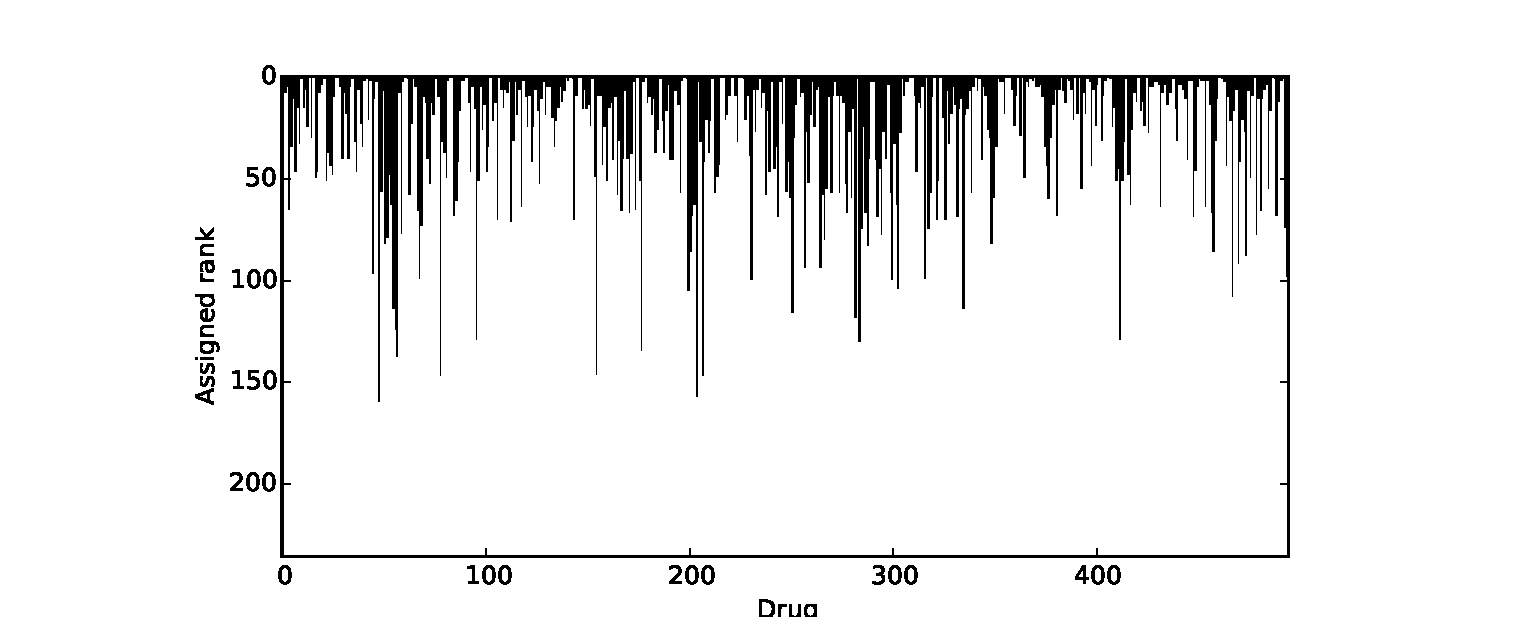
\includegraphics[width=\textwidth]{ref-ctd-heatmap.eps}
\caption{Reference CTD ``heatmap" where all pathways are inferred correctly}
\label{fig:ref-ctd-heatmap}
\end{figure}

To exactly quantify the performance of the model from such an image, metrics like precision and recall are used in information retrieval. 

Imagine covering all but the first line of the aforementioned ``heatmap" and then calculating the fraction of correctly predicted pathways that are visible (black squares) over all ``retrieved" pathways (all visible squares). This is the precision at that rank cutoff. The recall is defined as the fraction of correctly predicted pathways over all correct pathways (including the invisible ones, so the denominator is fixed for this dataset). Naturally, as more and more ranks get uncovered, the recall increases (since we're seeing more and more black squares), whereas the precision can vary (if all the newly uncovered squares are black, it will increase and if they are all white, it will decrease).

In the end of this process, multiple pairs of precision-recall values will be calculated and they can be used to plot a precision-recall curve.

One minor issue with this type of evaluation is that we essentially discard information by ranking pathways, since multiple distributions of pathways can map to the same ranking. In addition, we might prefer a pathway distribution where pathways that are not actually affected by the drug have lower expression values to the one where they are higher. For example, if a drug affects pathways 1 and 2 but not 3, and two models assign to this drug distributions $(0.4, 0.4, 0.2)$ and $(0.5, 0.4, 0.1)$, respectively, then the resultant pathway rankings are the same, but, intuitively, the second model seems to have made a better prediction in this case.

This intuition can be captured in the following measure:

\begin{equation}
c_d = \sum\limits_{p \in \mathit{ref}_d}{\theta_{d, p}}
\end{equation}

where $\mathit{ref}_d$ is a set of correct pathways for drug $d$ and $\theta_d$ is the predicted pathway distribution for drug $d$. Here, we find the proportion of activity that the model assigned to the pathways that are actually affected by the drug.

One question about this measure is whether we need to take into account the number of pathways the drug actually affects. In the most extreme example, if a drug affects all pathways in the dataset, any model will score a $1.0$ with this measure and so a model that scores 1.0 isn't necessarily ``good". On the other hand, if a drug only affects a single pathway and a model manages to assign $1.0$ to that pathway only, then the model's performance is impressive yet it scores $1.0$, as much as the previous case.

This is the reason comparison with random guessing is important: a random pathway distribution can be generated by drawing $K$ values from a uniform distribution and normalising them. On average, such a distribution will score $\rho_d$ on drug $d$, where $\rho_d$ is the drug's density (the fraction of pathways it actually affects). Hence, we can normalise the measure by dividing it by $\rho_d$ to find out by how much the model did better compared to random guessing. Furthermore, we can take the logarithm of this ratio so that the performance of random guessing ends up at 0, that of anything better than random gets a positive score and the performance of worse than random guessing becomes negative:

\begin{equation}\label{eq:rho-normalised-score}
M_d = \log(\frac{\sum\limits_{p \in \mathit{ref}_d}{\theta_{d, p}}}{\rho_d})
\end{equation}

This value will be referred as the rho-normalised log score further in the analysis.

\section{Toy datasets}

The following subsections describe the datasets which were generated and describes the results of the evaluation as per the aforementioned methods.

\subsection{Description of toy datasets}

The first batch of datasets was generated so that it mimics the properties of the real world KEGG/CMap dataset. All datasets from this batch have the following in common:

\begin{itemize}[noitemsep]
\item Vocabulary length (number of genes): 3000
\item Number of documents (drugs): 500
\item Number of words in each document: 1000
\item Density of $\beta$: 0.0138
\item Density of $\theta$: 0.1231
\end{itemize}

Densities here refer to the fraction of non-zero elements in each matrix. The KEGG/CMap dataset is very sparse: each pathway only affects, on average 1.38\% of all genes and each drug only affects, on average, 12.3\% of all pathways. The density value for $\beta$ was calculated by taking the matrix of priors (since it explicitly enforces the pattern of zeros in the result), whereas the density value for $\theta$ was calculated by taking the reference (CTD) dataset.

With these parameters, 5 datasets were generated:

\begin{itemize}[noitemsep]
\item 10 topics
\item 20 topics
\item 50 topics
\item 100 topics
\end{itemize}

These datasets allow to investigate how the performance of the model changes when the number of topics increases.

The parameters of the fifth dataset were designed to mimic the real-world one as closely as possible in order to determine, by comparing the performance of the model on that dataset against the real-world one, whether the drug gene expression data follows the generative framework described by the CTM. In addition to reusing all the parameters the first 4 datasets were generated with, for this dataset I also approximated the $\mu$ and $\Sigma$ of the reference by first calculating the topic distribution $\theta$ implied by the dataset (assuming all pathways in the resultant matrix are equally weighted) and then calculating the mean and the covariance matrix of the distribution of pathways based on it.

In the last 4 datasets, I varied the density of the covariance matrix: the proportion of pathways in the implied matrix of correlations that are connected:

\begin{itemize}[noitemsep]
\item No correlations: use the identity matrix as $\Sigma$
\item Density 10\%
\item Density 50\%
\item Density 90\%
\end{itemize}

\subsection{Convergence analysis}

TODO: ONE-ITERATION ANALYSIS (REDO ALL PLOTS)

At every iteration, the model outputs a likelihood bound that it assigns to the data and continues updating the model parameters until the likelihood bound converges (the change is less than a certain threshold). The likelihood bound values over iterations are plotted here.

It can be observed that increasing the number of topics decreases the likelihood bound the model assigns to the data and makes convergence slower.

\subsection{Topic prediction}

\begin{figure}[!htb]
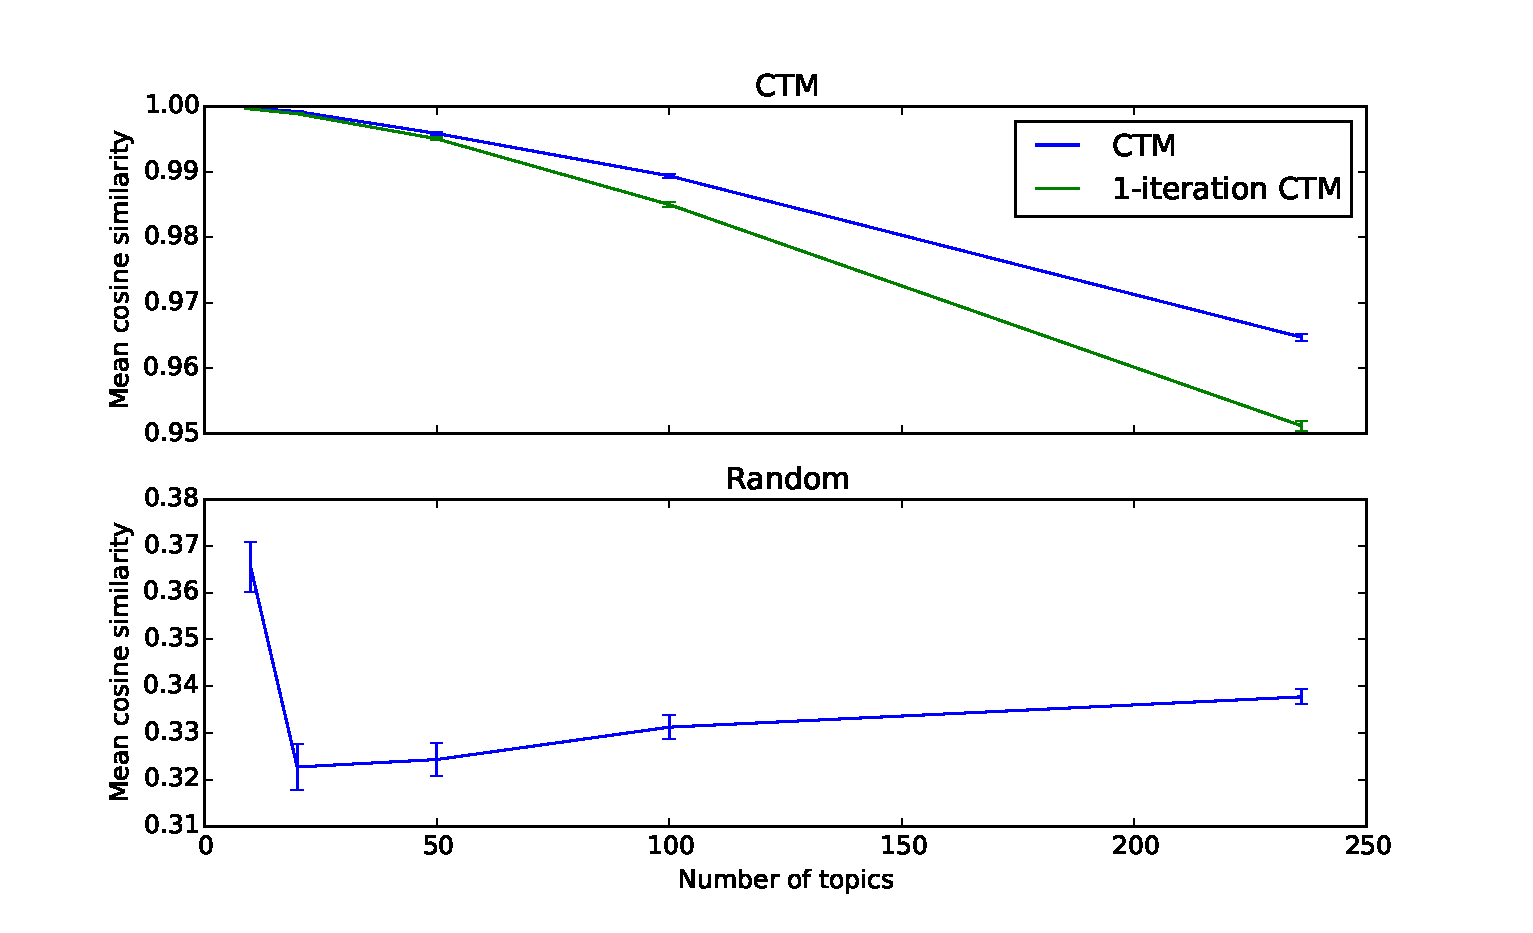
\includegraphics[width=\textwidth]{sim-cosine.eps}
\caption{The mean cosine similarity between inferred and reference topic distributions as a function of the number of topics in the toy datasets}
\label{fig:sim-cosine}
\end{figure}

In Figure~\ref{fig:sim-cosine}, dots on the plot denote the locations of the data points, since the error bars in this case are extremely small (the greatest sample error value on this dataset is 0.005 for the random guessing at $K=10$).

\subsection{Parameter recovery}

It would be reasonable to assume that if the model predicts the topic distribution for a document consistently well, it will also be able to recover the model parameters the corpus was generated with, since this is what the model relies on for its predictions. However, this is not exactly the case.

\begin{figure}[!htb]
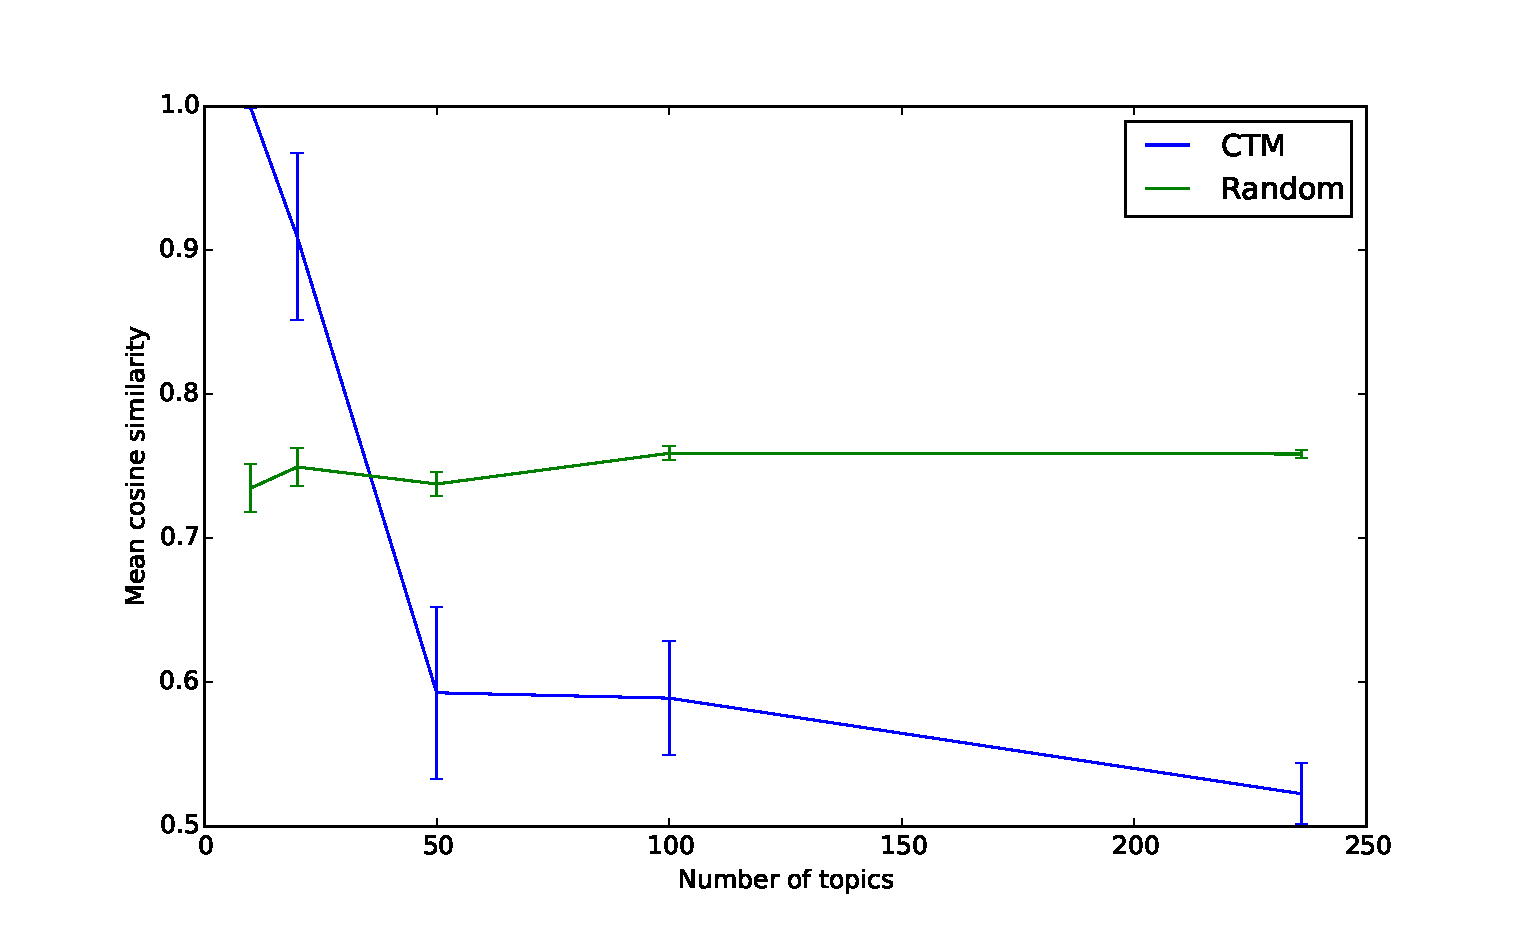
\includegraphics[width=\textwidth]{sim-beta-cosine.eps}
\caption{Cosine similarities between the inferred and reference topic-word distributions as a function of the number of topics in the toy datasets}
\label{fig:sim-beta-cosine}
\end{figure}

Figure~\ref{fig:sim-beta-cosine} shows the mean cosine similarity between the inferred and the reference rows of the $\beta$ matrix (the word distributions for every topic). There are $K$ topics in a single dataset and so every data point on this graph has been obtained by averaging the cosine similarities across $K$ samples. The random topic-word matrices here were generated by taking the Boolean matrix of priors and replacing the ``1" values with a draw from a uniform distribution and then renormalising.

As evident from the figure, the recovery of the topic-word matrix gets much worse as the number of topics increases and becomes further away from the reference than a random topic-word matrix after the third dataset. The reason for this is that the pattern of zeros in the resultant matrix differs from the matrix of priors even though the priors have been enforced. If the prior matrix contains a zero in a certain position, the inferred matrix is guaranteed to have a zero in the same position as well, since the zeros propagate through the training process. However, this doesn't mean that a zero in a certain position in the inferred matrix is also in the reference matrix. It appears that the training process can introduce a zero in certain positions and it will stay there throughout the remaining training iterations. This appears to be an issue of the topic recoverability and prior enforcement.

Another problem is the poor recoverability of the parameters of the global topic distribution, $\mu$ and $\Sigma$. The issue here is that every sample theta from $N(\mu, \Sigma)$ is altered after sampling by enforcing a certain number of zero elements. Hence, the document-topic distributions after generation are not guaranteed to follow a normal distribution with the original parameters. Intuitively, this is because theta values now have a larger chance of some elements coinciding (since they both have been set to zero), which introduces a bias into the correlations.

Despite all this, the model still achieves stellar performance in theta prediction tests on sparse datasets. This is because the theta prediction is dependent on not only the model parameters but also on the variational parameters, which take into account the actual words in the documents. Since with large numbers of topics the model parameters become useless for the theta prediction, there is no need to perform more than one variational inference iteration because further iterations will only change the global model parameters. I hence decided to evaluate the prediction performance of the model after just one iteration of training.

\subsection{Rank recovery}

\begin{figure}[!htb]
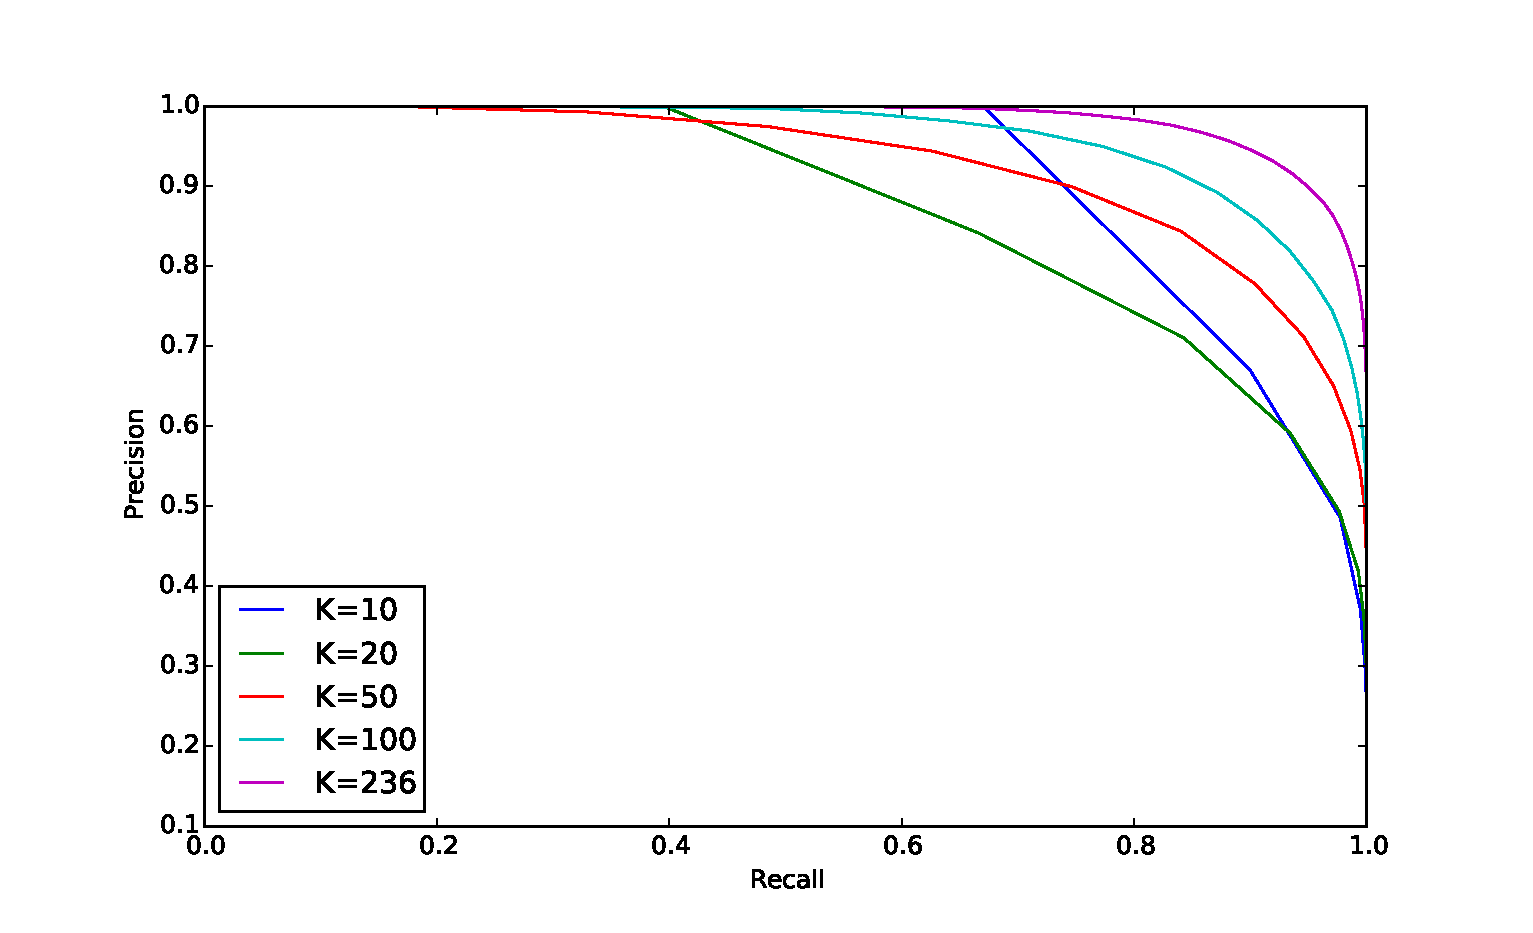
\includegraphics[width=\textwidth]{sim-pr-curves-all.eps}
\caption{Precision-recall curves for CTM on the toy datasets}
\label{fig:sim-pr-curves-all}
\end{figure}

TODO: add random baseline?

Figure~\ref{fig:sim-pr-curves-all} shows the precision-recall curves for the toy datasets with different number of topics on the same axis. The reference precision-recall curves (where all relevant topics/pathways are in the top ranks) can also be plotted, but in this case the CTM curves are so close to the reference curves they are indistinguishable. However, the topic recovery of CTM is not perfect, according to the previous tests, so a different method has to be used to evaluate how CTM fares on ranked retrieval tasks.

\begin{figure}[!htb]
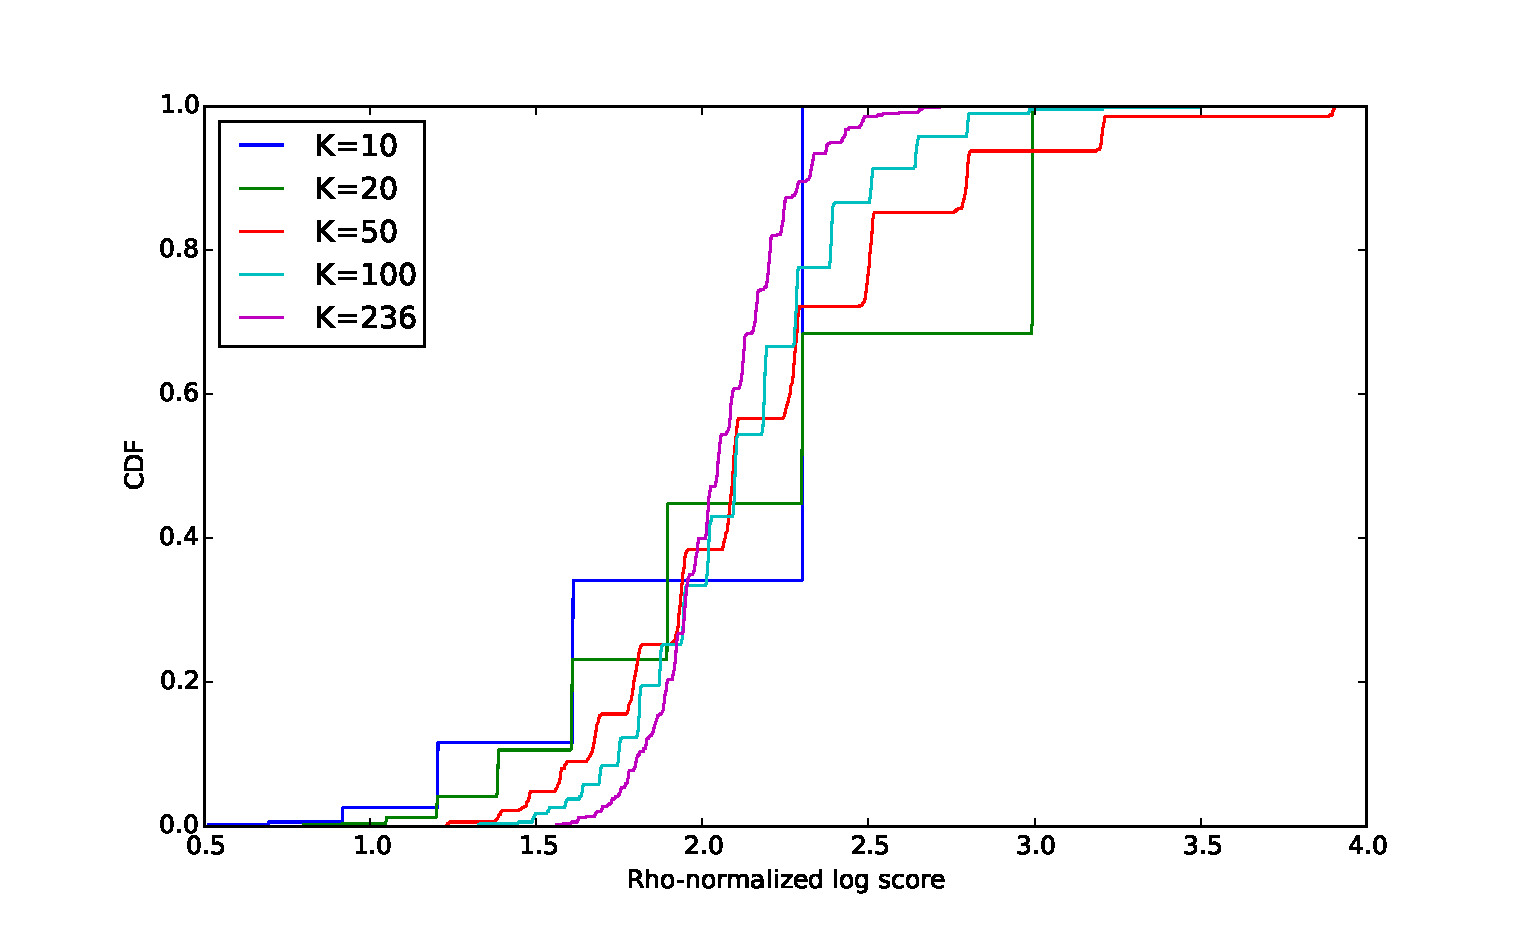
\includegraphics[width=\textwidth]{sim-log.eps}
\caption{CDF of the distribution of the rho-normalised log scores of CTM on the toy datasets}
\label{fig:sim-log}
\end{figure}

Figure~\ref{fig:sim-log} shows the cumulative plots of rho-normalised log scores (Equation~\ref{eq:rho-normalised-score}) as the number of topics changes. While these plots do show that the CTM gives a much better performance than random guessing (since all scores are above 0), the figure is too confusing for any conclusions to be made. It does, however, show an interesting ``staircase" effect where the scores fall into discrete bins whose amount increases with the number of topics. This is because the unnormalised measure (sum of inferred expression levels for correct pathways) is close to 1 and so the final score only depends on the normalisation factor, which only depends on the number of pathways the drug actually has.

\begin{figure}[!htb]
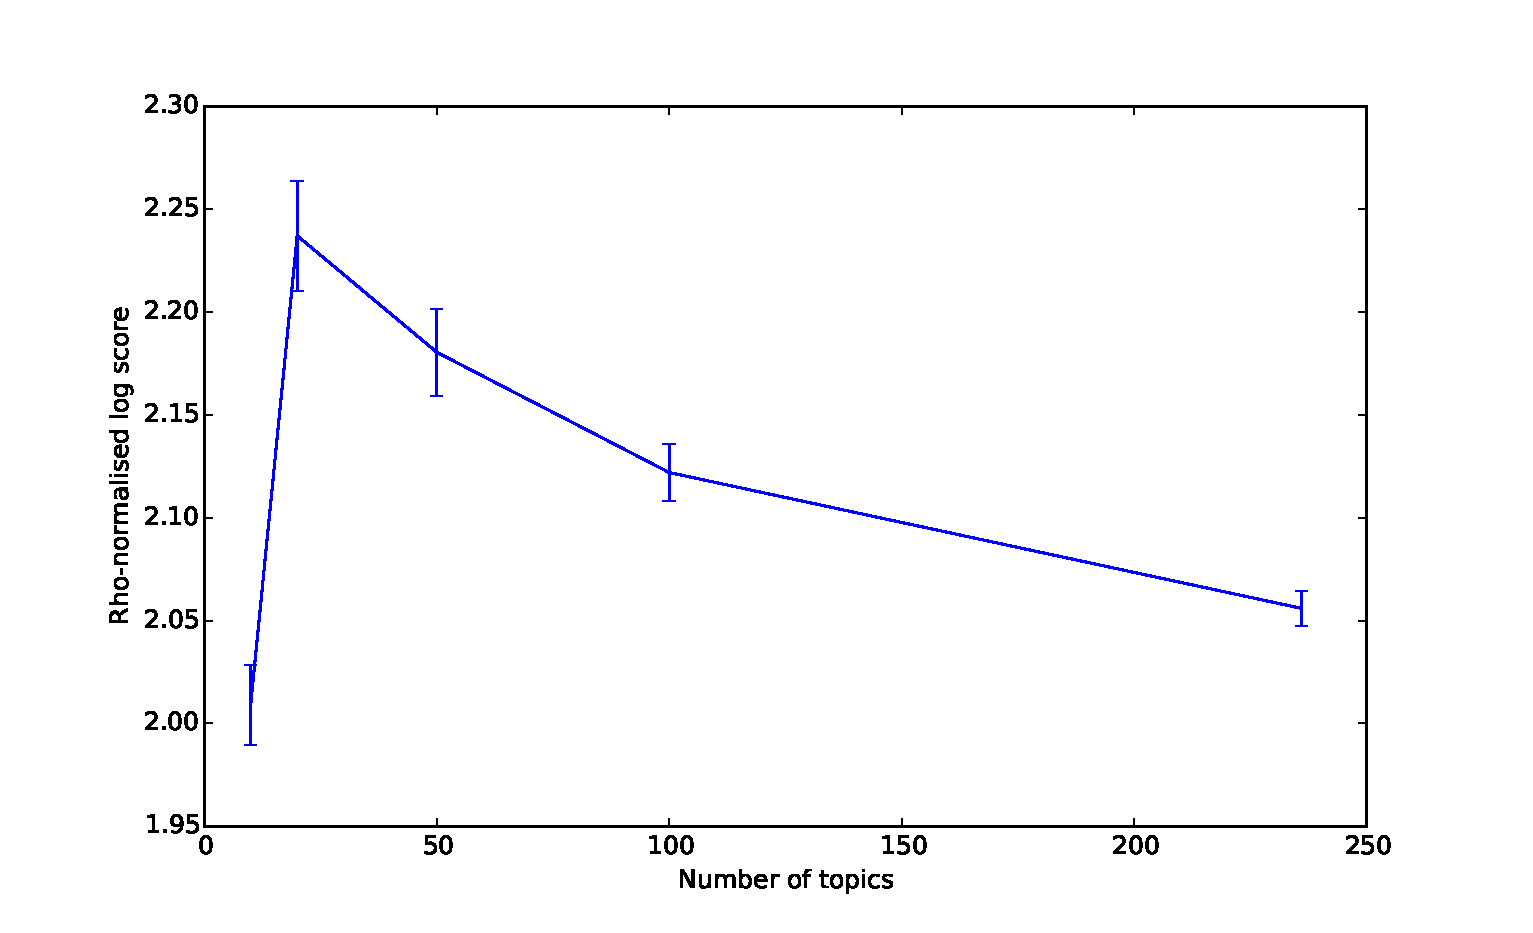
\includegraphics[width=\textwidth]{sim-average-rho.eps}
\caption{Average rho-normalised log score as a function of the number of topics in the toy datasets}
\label{fig:sim-average-rho}
\end{figure}

Figure~\ref{fig:sim-average-rho} shows the mean score the model achieved on every dataset, plotted against the number of topics. The performance of the model generally degrades with the number of topics, however there is a peak somewhere between $K=10$ and $K=50$ where the model achieves top performance.

\section{KEGG and CMap datasets}

\subsection{Description of the dataset}

KEGG (Kyoto Encyclopedia of Genes and Genomes), published by Kyoto Universiy Katehisa Laboratories, is an online collection of databases dealing with various aspects of biology. Of interest to this project is the KEGG PATHWAY database, a collection of pathways and genes which they include.

CMap (Connectivity Map), published by the Broad Institute is a catalog of gene-expression data.

These two datasets are used to derive the following matrices:

\begin{itemize}[noitemsep]
\item Drug-gene expression matrix, where each entry is the logarithm of the ratio of the expression of the gene when treated with a certain drug against the baseline, rounded to 2 decimal places.
\item Boolean gene-pathway membership matrix that has a ``1" entry if the pathway contains a given gene and ``0" if it doesn't.
\end{itemize}

I used the same preprocessed data that was used in the LDA paper, so I didn't have to perform the preprocessing of the raw gene expression data myself. This was so that the results from the LDA and the CTM method could be compared.

Before the CTM can be trained on the dataset, the drug-gene expression data has to be turned into a sort of a ``document", since we're now operating in terms of words and word counts. Both LDA and my implementation of CTM do it by taking the absolute value of each element and multiplying it by 100 (since the preprocessed data has been rounded to the nearest 0.01). Observe that this discards the sign of the expression value and since we're operating in log space, this means that the gene expression ratios that are reciprocals of each other will be treated the same.

I was not comfortable with this method since it involved discarding information that the model might have had a use for, but the CTM training process does require nonnegative values. I hence performed another experimental run where the differential gene expression data was exponentiated (since the source matrix actually has logarithms of the gene expression ratio). It will be referred to here as ``CTM with exponentiation".

The parameters of the training dataset are:
\begin{itemize}[noitemsep]
\item 3041 gene
\item 236 pathways
\item 1169 drugs
\item Density of $\beta$: 0.0138
\item Density of $\theta$: 0.1231
\end{itemize}

It took about 9 hours to train the model on the whole dataset and perform the inference of the pathway structure for every drug.

TODO: CTM inference had 1000 theta samples, enough?

To perform a quick sanity check for the results, I took the cosine similarities for the predicted pathway distributions by CTM and LDA for every drug and plotted their distribution (Figure~\ref{fig:ctd-ctm-lda-diffs}). The distribution of cosine similarities between random guessing and LDA is also plotted for comparison. It can be seen that CTM and LDA give very similar results.

\begin{figure}[!htb]
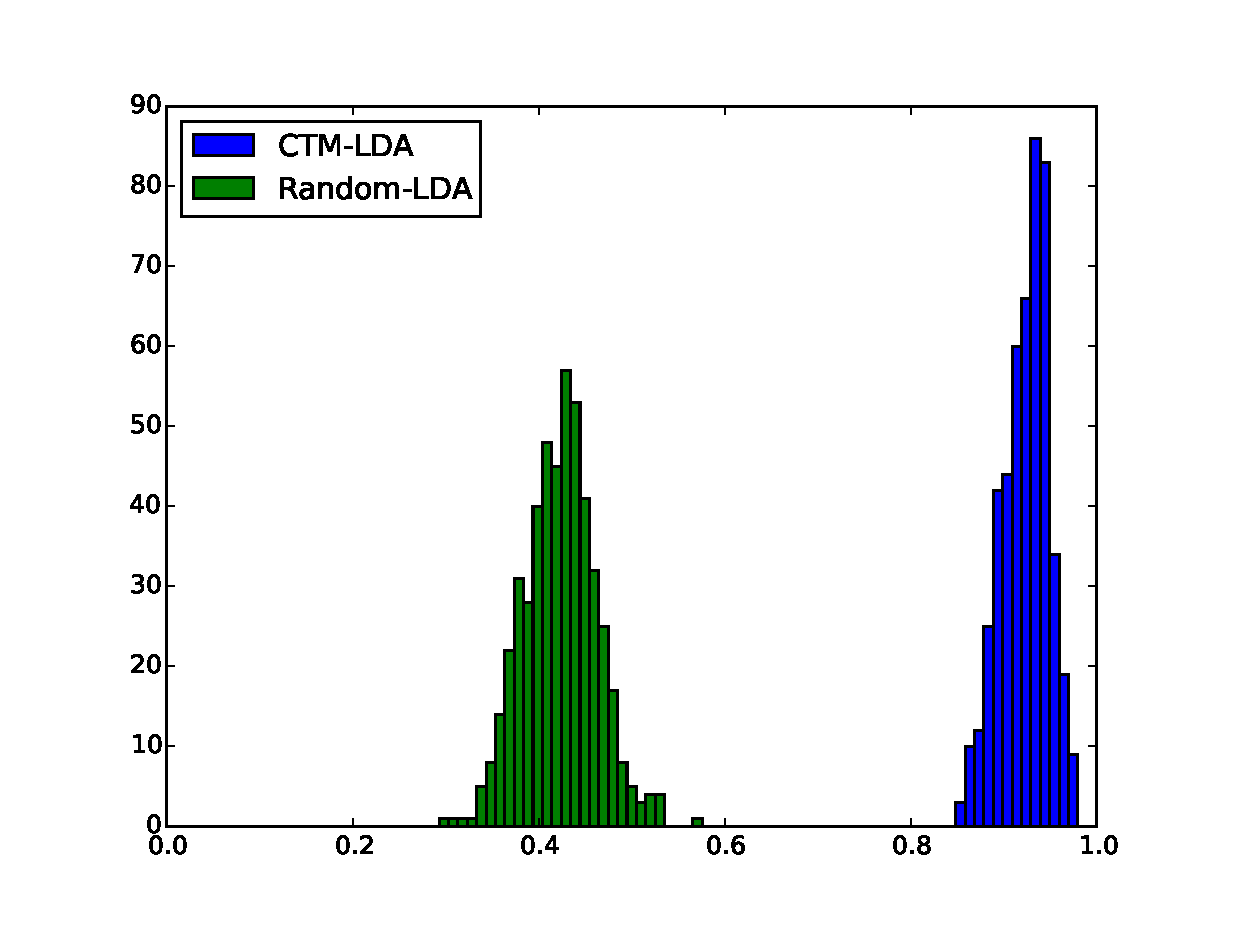
\includegraphics[width=\textwidth]{ctd-ctm-lda-diffs.eps}
\caption{Histogram of the cosine similarities between the topics inferred by CTM and LDA}
\label{fig:ctd-ctm-lda-diffs}
\end{figure}

\subsection{CTD}

TODO: What is CTD?

The CTD dataset is a catalogue of drugs that lists which pathway each one of those affects. Not all pathways and not all drugs used in the KEGG/CMap dataset are mentioned in the CTD, so thefinal drug-pathway prediction matrices output by LDA and CTM had to be filtered down to the shape of CTD: 495 drugs (thus simply dropping the relevant rows) and 193 pathways (removing the columns and renormalising).

The predicted thetas are then used to rank the pathways for every drug.

Figure~\ref{fig:ctm-ctd-heatmap} shows a so-called ``heatmap" for CTM, explained in the beginning of this section.

\begin{figure}[!htb]
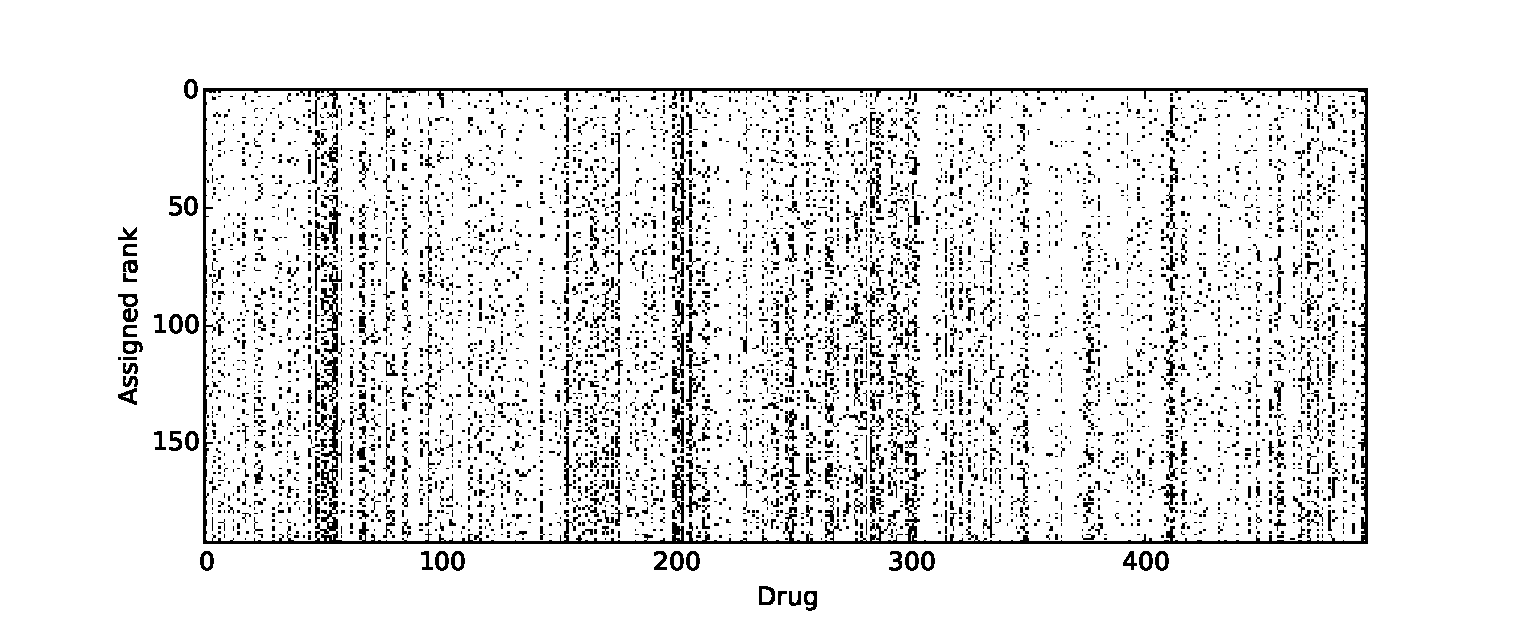
\includegraphics[width=\textwidth]{ctm-ctd-heatmap.eps}
\caption{CTD ``heatmap" for CTM}
\label{fig:ctm-ctd-heatmap}
\end{figure}

\begin{figure}[!htb]
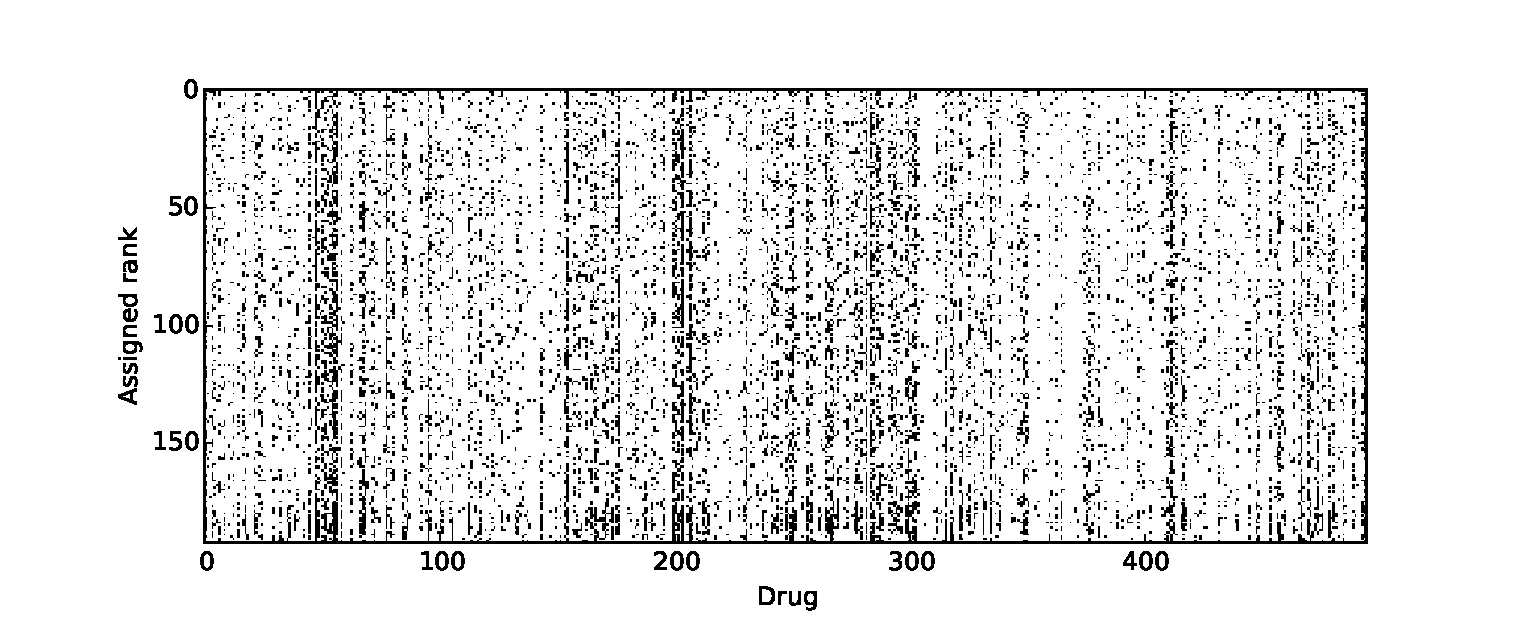
\includegraphics[width=\textwidth]{lda-ctd-heatmap.eps}
\caption{CTD ``heatmap" for LDA}
\label{fig:lda-ctd-heatmap}
\end{figure}

The expected behaviour is for the black squares to cluster towards the top of the ``heatmap", since that means the model assigned the top ranks to pathways that are actually correct. However, both LDA (Figure~\ref{fig:lda-ctd-heatmap}) and CTM are very far from that and to see exactly how, a different visualisation is required.

\subsubsection{Precision-recall curves}

The precision-recall curves for the whole dataset are plotted in Figure~\ref{fig:ctd-pr-curves}.

\begin{figure}[!htb]
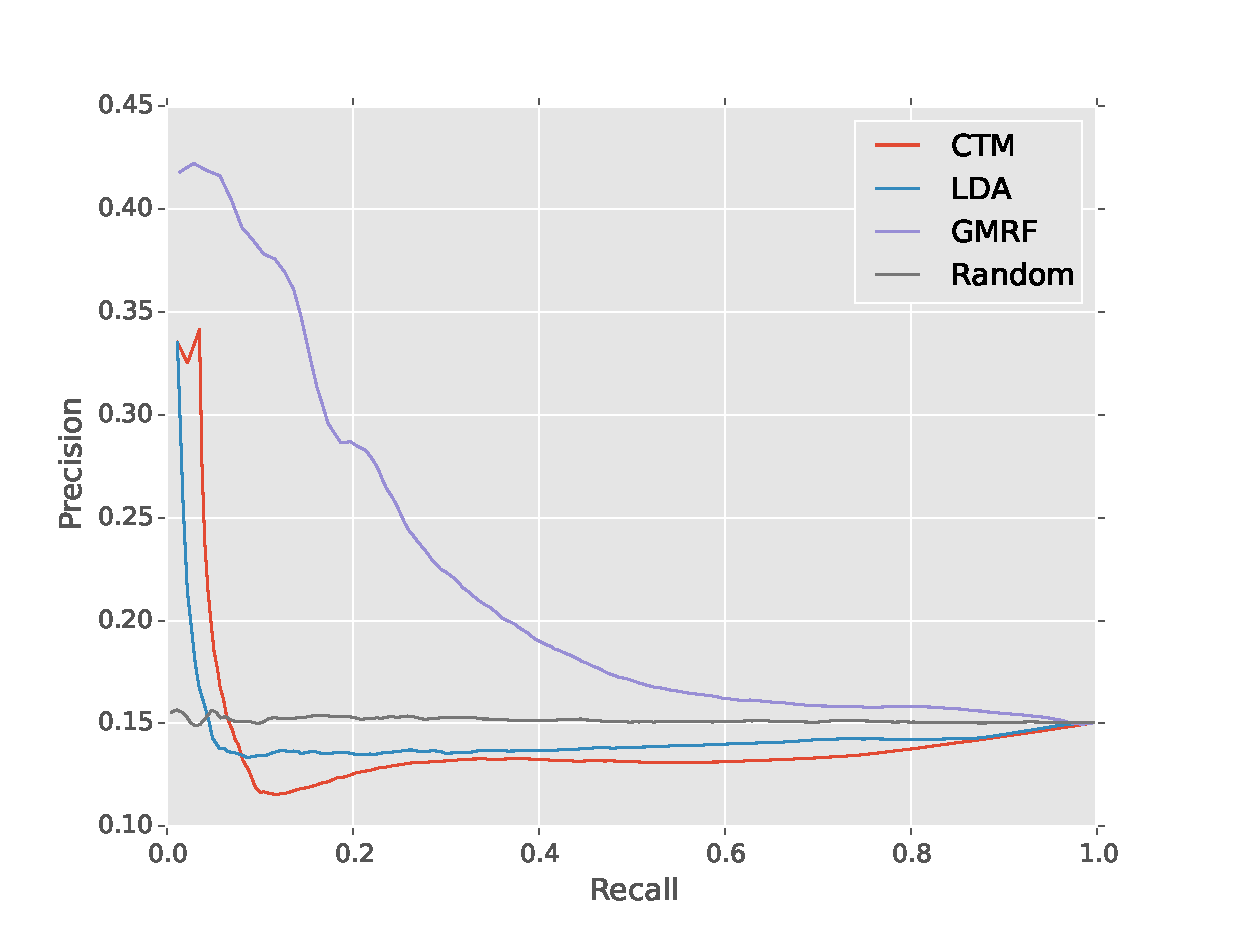
\includegraphics[width=\textwidth]{ctd-pr-curves.eps}
\caption{Precision-recall curves on the validation dataset (CTD) for CTM, LDA, and random topic assignments (baseline)}
\label{fig:ctd-pr-curves}
\end{figure}

The MAP values for CTM, LDA and CTM with exponentiation are 0.181, 0.189 and 0.204, respectively. The average MAP value for random guessing is 0.172.

The main conclusion to be made from this is that while CTM does have some predictive power, since its performance is significantly different from the baseline, it, in fact, does not outperform LDA on this dataset. Exponentiating the gene expression data prior to training (and thus not discarding the sign), however, improves the performance of CTM beyond that of LDA.

One curious phenomenon on this graph is the large spike in precision at low recall levels, meaning that all models made multiple correct predictions at top ranks. Figure~\ref{fig:ctd-side-plot-10} shows this in more detail: it plots, in essence, the number of black squares in each model's ``heatmap" at every rank up to 10. For almost half of all the drugs, the three models' most expressed pathway is indeed confirmed by CTD to be affected by those drugs.

\begin{figure}[!htb]
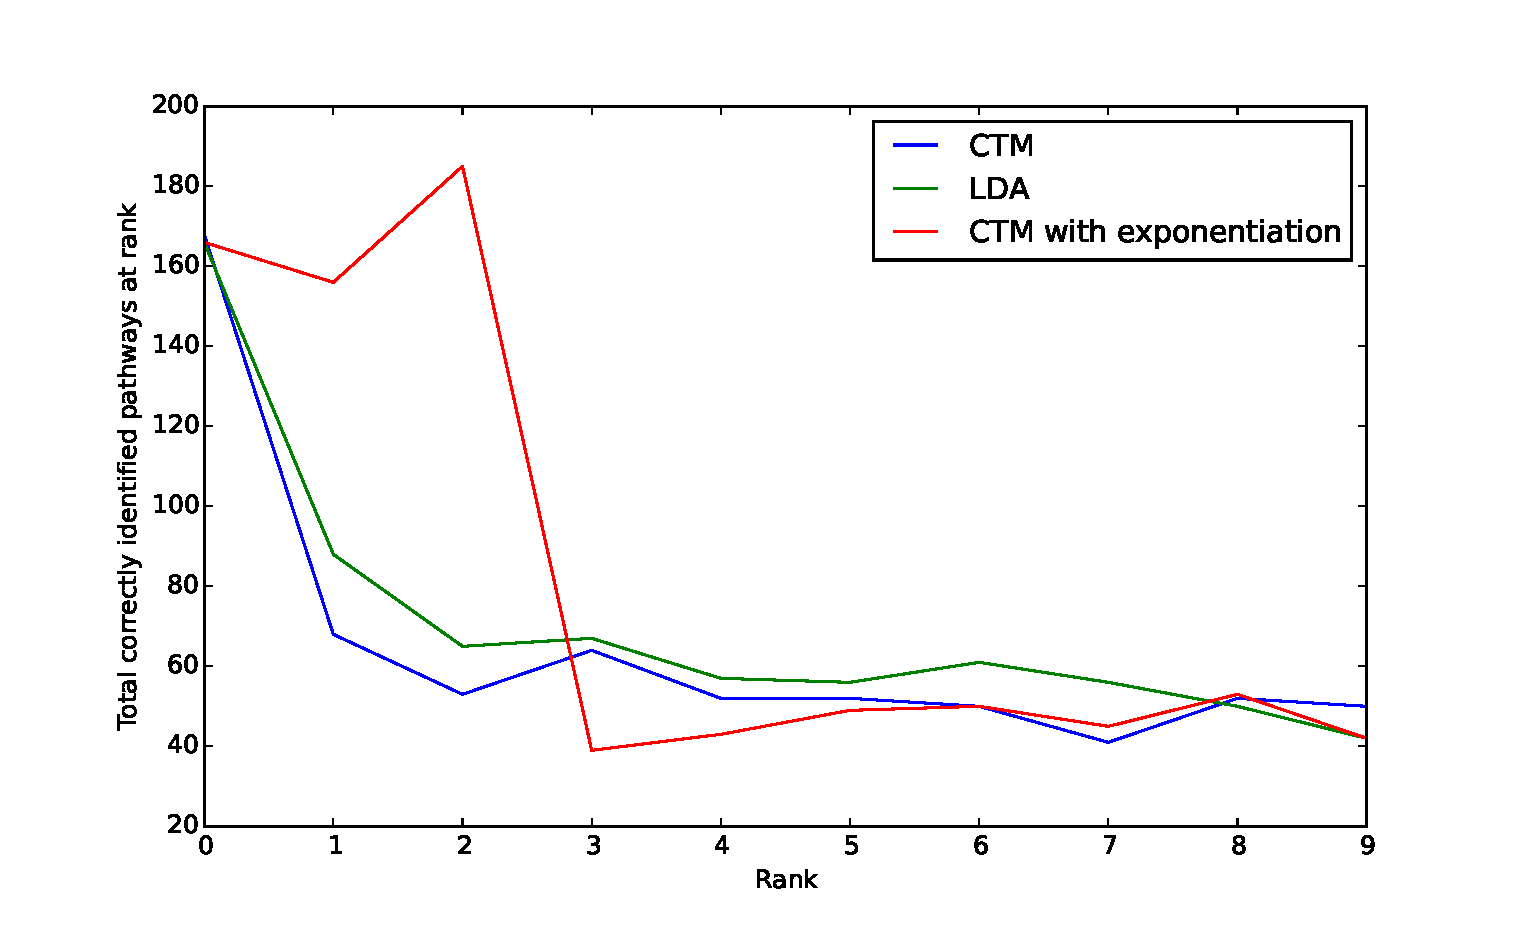
\includegraphics[width=\textwidth]{ctd-side-plot-10.eps}
\caption{Number of drugs with correctly identified pathways at each rank.}
\label{fig:ctd-side-plot-10}
\end{figure}

Closer inspection, however, reveals that the three models rank a pathway named ``Metabolic pathways" as first for most drugs in the evaluation set (495 (all drugs) for LDA, 480 for CTM and 474 for CTM with exponentiation). This pathway is a ``catch-all" for all metabolic pathways, uniting all pathways in the dataset. Ignoring it in the evaluation process changes the results tremendously.

\begin{figure}[!htb]
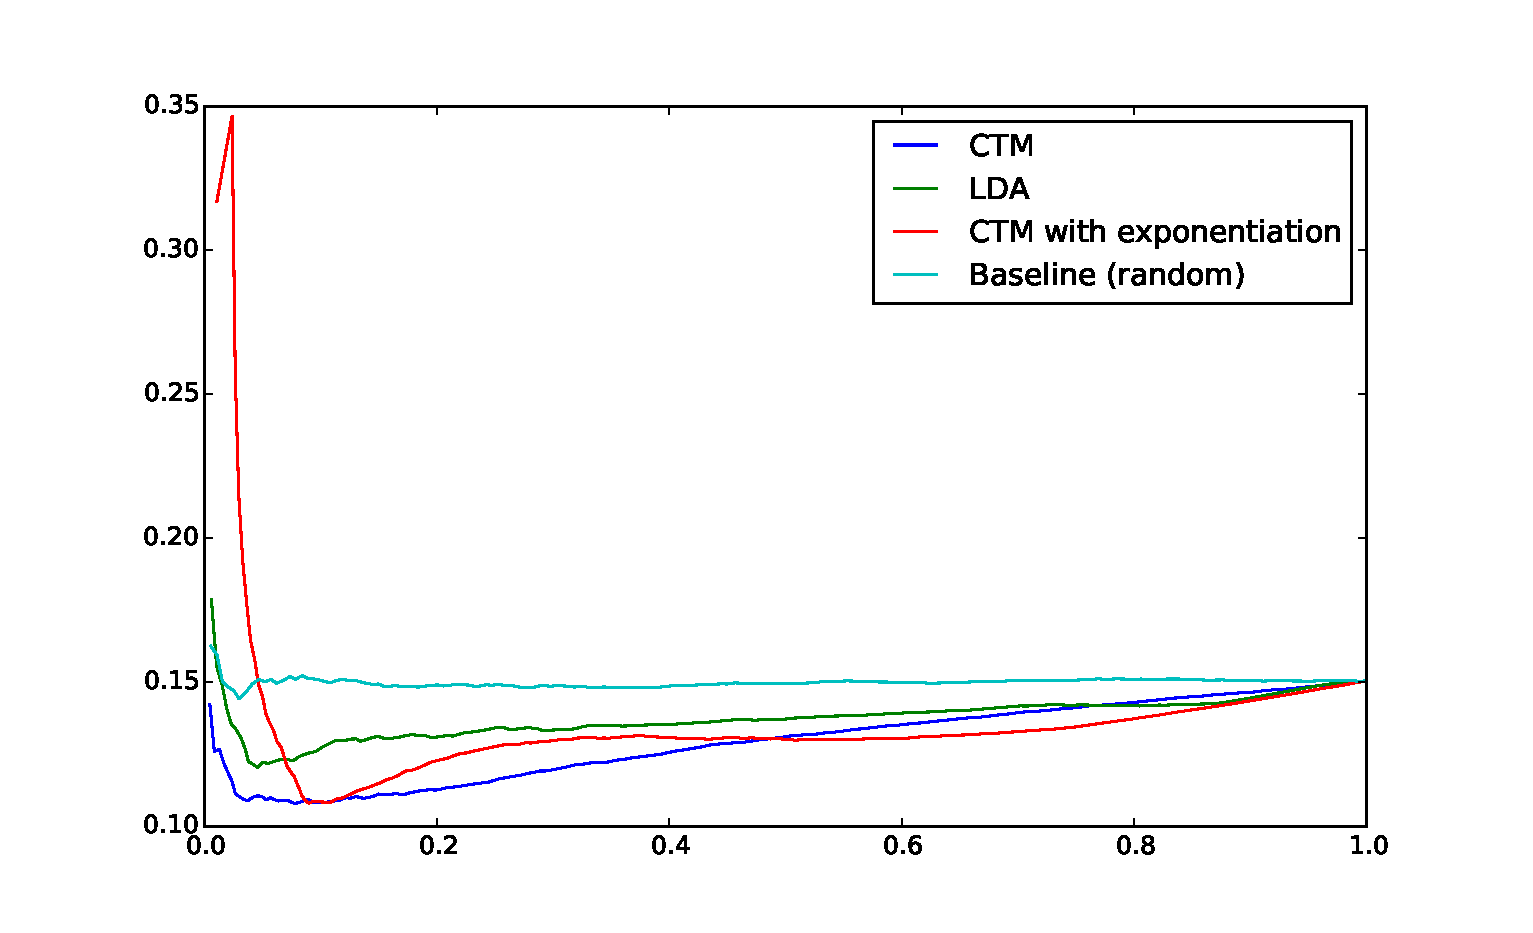
\includegraphics[width=\textwidth]{ctd-pr-curves-no1100.eps}
\caption{Precision-recall curves on the validation dataset with the ``Metabolic pathways" pathway excluded.}
\label{fig:ctd-pr-curves-no1100}
\end{figure}

Figure~\ref{fig:ctd-pr-curves-no1100} shows the resultant precision-recall curve. The new MAP values for CTM, LDA and CTM with exponentiation are 0.176, 0.166 and 0.213, respectively whereas the random method achieves a MAP value of 0.172. LDA still beats CTM and the fact that CTM relied on the presence of the removed pathway for most of its performance now has dropped its MAP value below that of random guessing. However, CTM with exponentiation now vastly outperforms all the other models.

\subsubsection{Rho-normalised log scores}
Figure~\ref{fig:ctd-rho-cdf} shows the CDF plots of the rho-normalised log scores (Equation~\ref{eq:rho-normalised-score}) for CTM, LDA and CTM with exponentiation (with the ``Metabolic pathways" pathway excluded). It can be seen from the plot that the median score of all three models is below that of random guessing. The parameters of this distribution are summarised in table~\ref{tab:ctm-ctf-summary}. The performance of random in this case was obtained by simulating 1000 random drug-pathway distributions and averaging their mean performance.

\begin{figure}[!htb]
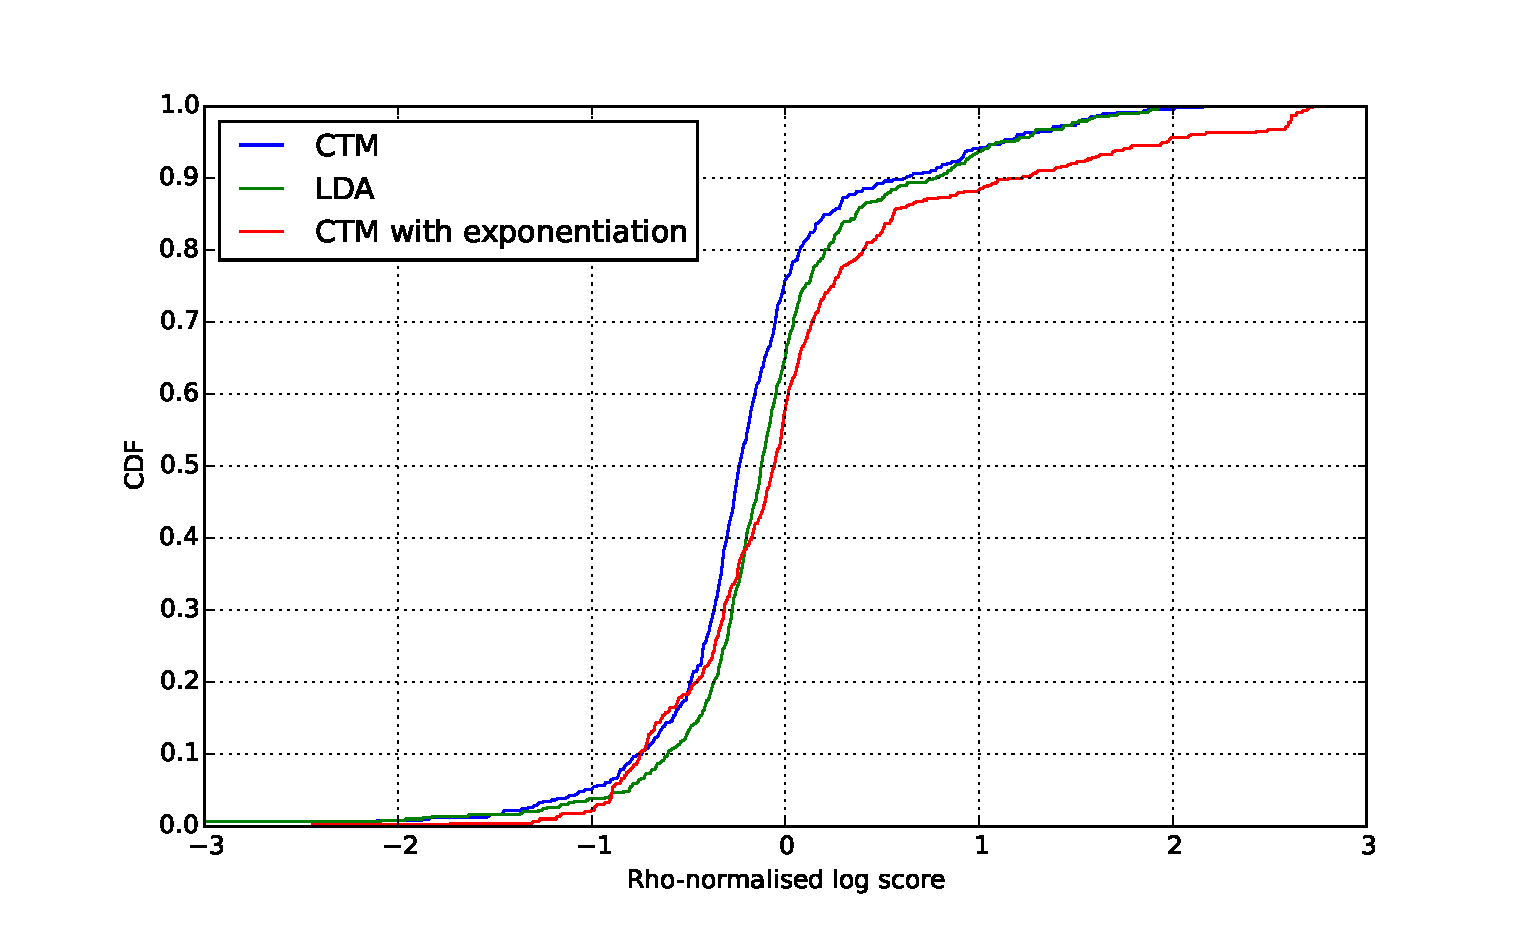
\includegraphics[width=\textwidth]{ctd-rho-cdf.eps}
\caption{CDF of the rho-normalised log score of the models on the CTD data}
\label{fig:ctd-rho-cdf}
\end{figure}

\begin{table}
\begin{tabular}{| l | l | l | l |}
\hline
Model & Mean & Median & Standard deviation\\
\hline
CTM & -0.177 & -0.238 & 0.654 \\
LDA & -0.070 & -0.125 & 0.645 \\
CTM with exponentiation & 0.064 & -0.059 & 0.801 \\
Random & -0.008 & 0.000 & 0.124 \\
\hline
\end{tabular}
\caption{Parameters of the distribution of the rho-normalised log scores}
\label{tab:ctm-ctf-summary}
\end{table}

CTM with exponentiation is the only method that achieved a positive mean score, since its performance distribution has a heavy right tail: about 10\% of its predictions achieved a score greater than 1.

\subsubsection{Clustering the drug similarity matrix}
Since the document (or drug) similarity matrix (\ref{eq:document_similarity_matrix}) is not affected by the topic identifiability, I decided to perform clustering on the matrix to identify some common groups of drugs and reference them to the actual descriptions of those drugs.
I used the Markov Clustering Algorithm (MCL)  \cite{Dongen:2000:CAG:868986}, a simple method that's based on the insight that a document similarity matrix, when normalised, forms a Markov chain. If one simulates multiple ``random walkers" on this chain and slowly starts weakening the links between the elements of the chain, each of them will eventually end up roaming around the final clusters. This is encoded in the following algorithm:

\documentclass{article}
\usepackage[noend]{algpseudocode}
\usepackage[]{algorithm}
\usepackage{amsmath}
\usepackage[cm]{fullpage}
\newcommand{\var}[1]{{\operatorname{\mathit{#1}}}}

\begin{document}
\begin{algorithm}
	\caption{Markov Clustering Algorithm}
	\label{markov-clustering}
	\begin{algorithmic}[0]
		\Function{markov-clustering}{$M, \var{expansion}, \var{inflation}$}
			\While{change in $M >$ threshold}
				\State Normalize $M$
				\State Expansion step: $M \gets M^{\var{expansion}}$
				\State Inflation step: $M_{i,j} \gets M_{i,j}^{\var{inflation}}$
			\EndWhile
			\State Normalize $M$
			\State\Return $M$
		\EndFunction
	\end{algorithmic}
\end{algorithm}

\end{document}

The algorithm consists of repeatedly performing expansion and inflation on the transition matrix: in the expansion step, we exponentiate every element of the matrix (thus weakening the links between different elements) and in the inflation step, we exponentiate the matrix itself (thus turning it into an $\mathit{inflation}$-step transition matrix and simulating the ``random walkers").

This process is guaranteed to converge on most graphs and the result can be interpreted as follows: if $M_{i,j} > 0$, then $j$ is a member of the cluster whose main ``attractor" is $i$. This value will usually be 1, meaning each element can only be a member of one cluster, but in case of some symmetric graphs it can be a fraction.

todo: about expansion/inflation parameters

\subsection{ATC classification}

Drugs have a hierarchical code that depends on what they actually do (example). This code is possible to predict from the gene expression data by training a generic classifier on it.

If the inferred pathway proportions from the models are used instead as inputs, is the performance better?

\subsection{Drug-target prediction}

\chapter{Conclusion}

%%%%%%%%%%%%%%%%%%%%%%%%%%%%%%%%%%%%%%%%%%%%%%%%%%%%%%%%%%%%%%%%%%%%%
% the bibliography
\addcontentsline{toc}{chapter}{Bibliography}
\bibliography{bibliography}

%%%%%%%%%%%%%%%%%%%%%%%%%%%%%%%%%%%%%%%%%%%%%%%%%%%%%%%%%%%%%%%%%%%%%
% the appendices
\appendix

\chapter{Project Proposal}

\documentclass[12pt,a4]{article}
\usepackage{hyperref}
\usepackage{color}
\usepackage{fullpage}
\begin{document}

\vfil


\begin{flushright}
\large{A. I\v{s}kovs}\\
\texttt{ai280}\\
Trinity College
\end{flushright}

\vspace*{\fill}
\begin{center}{\large Computer Science Tripos, Part II Project Proposal}

\vspace{0.3in}
\textbf{\center{\Large Predicting drug-pathway interactions using the Correlated Topic Model}}

\vspace{0.4in}
\centerline{\large \today}
\end{center}
\vspace*{\fill}

\vfil

%
%\noindent{\bf Project Originator:} N. Pratanwanich
%\vspace{0.4in}
%
%\noindent
%{\bf Project Supervisor:} N. Pratanwanich\\
%
%\noindent
%{\bf Signature:}
%\vspace{0.2in}
%
%\noindent
%{\bf Director of Studies:} Dr A. C. Norman\\
%
%\noindent
%{\bf Signature:}
%\vspace{0.2in}
% 
%\noindent
%{\bf Project Overseers:} Dr~A.~V.~S.~Madhavapeddy  \& Dr~S.~H.~Teuffel\\
%
%\noindent
%{\bf Signatures:}

\pagebreak

% Main document

\section*{Introduction}

Latent Dirichlet Allocation\cite{Blei} is a bag-of-words topic modelling algorithm that treats documents in a corpus as being generated by picking a set of topics and then drawing words from those topics. Using a sampling method, the posterior distributions of unknown variables (probability distributions of topics and words within topics) are inferred. This allows, for an arbitrary document, to infer a probability distribution of topics which it is about.

The 2014 paper\cite{Pratanwanich2014} by Naruemon Pratanwanich and Pietro Lio describes a model based on this algorithm to predict drug-pathway relationships: differential gene expression profiles of drug treatments are treated as documents, pathways where genes are functionally grouped as topics and genes as words. The model had to be augmented with priors: the pathway-gene relationships for some pathways are already known. In the end, this method provided better predictive results of pathways activated by certain drugs than the state-of-the art methods.

A problem with Latent Dirichlet Allocation and hence this approach is that it assumes that the topics (or pathways) are uncorrelated. This assumption is usually not true: a document about Computer Science is more likely to be about Mathematics than, say, Geology. Another 2014 paper\cite{C4MB00014E} by Naruemon Pratanwanich and Pietro Lio presents a model that assumes pathway crosstalk (correlation). It uses matrix factorisation together with this assumption to predict pathway responsiveness for drugs that affect multiple pathways and finds that using the correlation assumption results in a better fit to the gene expression data.

The Correlated Topic Model\cite{2007} was proposed as an improvement on the Latent Dirichlet Allocation: instead of using the Dirichlet distribution to model the relative proportions of topics in a document, it uses the logistic normal distribution. The parameters of the distribution are the mean and the covariance matrix, which allows for modelling correlations between topics. The original paper\cite{2007} uses a deterministic approach called Variational EM (Expectation Maximization) to train this model (due to the non-conjugacy of the logistic normal, the Markov Chain Monte Carlo approach with Gibbs Sampling is intractable). The Correlated Topic Model fit the sample corpus (a set of articles from \textit{Science}) better than LDA\cite{2007}.

Since the matrix factorization model that assumed pathway correlation\cite{C4MB00014E} and the LDA method\cite{Pratanwanich2014} outperform matrix factorization without correlations, it is suspected that adapting the CTM to the problem of prediction of pathway responsiveness to drug treatment would yield another improvement in predictive power.

The aim of this project is to implement and test such a model. In addition to reusing the Bayesian network from the CTM, the model will be augmented with a prior distribution of known gene-pathway relationships. The equations for training the model will be derived, based on the existing CTM equations for Variational EM\cite{2007}. The model will be tested on a synthetic corpus of drug gene expression data for model verification and then on publically available datasets (CMAP\cite{CMap} for gene expression data and KEGG\cite{KEGG} for pathway data). The results will be compared with the latent variables inferred by the LDA approach. While it's not possible to guarantee that the model will perform better in every case, the results will be investigated to see in which cases the LDA approach performs better than CTM and vice versa.

\section*{Starting Point}

I know Python and have some experience in working with the SciPy stack. Python has lots of facilities for data processing and while it is an interpreted language, NumPy uses native LAPACK/BLAS (linear algebra) libraries as a backend. This means that the performance of the linear algebra routines is on par with C.

Since this project uses some concepts from the Artificial Intelligence II course (see Key Concepts), I will have to familiarise myself with the course before it begins.

There exists an R package for the Correlated Topic Model, as well as a C implementation of the Model written by the authors of the original paper (\url{https://www.cs.princeton.edu/~blei/ctm-c/}). I will however only be able to use those as a reference at most: adding priors to the model will change its implementation. On the other hand, the C implementation has a way to perform posterior inference (prediction) on new documents, which can help with one of the extensions to the project.

\section*{Substance and Structure of the Project}

\subsection*{Key Concepts}

The key concepts in this project are drawn from the Artificial Intelligence II course, including topics such as Bayesian Networks and inference, methods for training and evaluating classifiers and probability distribution transformation. This project, however, will go beyond the scope of the course, touching on Variational Inference, conjugate and non-conjugate distributions and Expectation Maximization.

\subsection*{Major Work Items}

\subsubsection*{Required Reading and Research}

\begin{itemize}
\item Artificial Intelligence II Lecture notes: introduction to Bayesian networks and inference
\item Chapters 9 and 10 of Christopher Bishop's book\cite{Bishop:2006:PRM:1162264} on computer vision models: Mixture models (of which LDA and CTM are variations) and the Expectation Maximization algorithm, as well as Variational Inference.
\item ``Build, Compute, Critique, Repeat: Data Analysis with Latent Variable Models"\cite{doi:10.1146/annurev-statistics-022513-115657}, an introduction to latent variable models that describes how to train the models using mean-field Variational Inference, use them to perform predictions and evaluate them.
\item The original LDA\cite{Blei} and CTM\cite{2007} papers to understand the structures of the respective generative probabilistic models and their inference based on Variational EM.
\item Naruemon Pratanwanich and Pietro Lio's paper\cite{Pratanwanich2014}  on adapting LDA in order to familiarize myself with how microarray data is preprocessed into a pseudo-drug ``document", how the gene-pathway membership priors are incorporated into the model, as well as the ranking method used to evaluate its performance.

I will also need to get a better understanding of the biological context around the project, including topics such as genes, pathways, how the drug gene expression data is obtained using microarrays and how it has to be preprocessed.

\end{itemize}

\subsubsection*{Developing a Model}

The classic Expectation Maximization algorithm consists of two steps:

\begin{itemize}
\item \textbf{E}: Calculate the expected value of the log likelihood of seeing the latent variables given the observed variables and the model parameters.
\item \textbf{M}: Maximize this function by updating the model parameters.
\end{itemize}

The CTM paper\cite{2007} applies an algorithm called Variational EM that, using a variational distribution, approximates the posterior distributions of latent variables with respect to the model parameters in the \textbf{E} step and estimates the model parameters with respect to variational parameters in the \textbf{M} step.

I have to understand and alter this algorithm in order add prior information on gene-pathway memberships to the model.

\subsubsection*{Implementation and Testing}

In Python, implement:

\begin{itemize}
\item The software to generate synthetic data for model verification and to preprocess real datasets.
\item The actual Correlated Topic Model that incorporates the priors.
\end{itemize}

During development, the model will be tested using toy datasets of synthetic gene expression and pathway data. Using the real datasets, it will then be compared against the LDA method (see Evaluation and Success Criteria).

\subsubsection*{Fallback Plan}
In case I fail to incorporate priors into the Correlated Topic Model, I will use one of the available libraries for fitting the CTM and instead work on processing the gene data into a drug "document" that can be understood by the library, as well as developing a way to predict pathway distributions for a previously unseen drug. The evaluation procedure in that case will have to be changed, since not having priors in the model will mean that the pathways will be completely arbitrary and will not correspond to real drug data.

Another option is using a less complicated algorithm such as Random Forests that has high predictive power on drug-pathway perturbations\cite{Riddick15012011}. In that case the setting will be that of supervised learning, where the training data are known pairs of drugs and pathways and the features are the differential gene expression data. However, in this case I won't be able to test the hypothesis of pathway correlation and how the data are generated as I would be able to by using the aforementioned generative probabilistic models.

\section*{Evaluation and Success Criteria}

The \textbf{main criterion} for success is a working implementation of the model as per its specification. This will be evaluated as follows:
\begin{itemize} 
\item Generate a toy dataset of random pathways, pathway-gene memberships (a probability distribution over genes) and drug-pathway interactions (a probability distribution over pathways)
\item Use that to generate a corpus of gene expression data as per how the Correlated Topic Model assumes it's generated.
\item Together with a random subset of the pathway-gene membership data to serve as a prior, use the model to infer the latent variables and compare them with the ones that generated the dataset.
\end{itemize}

Note that the successful achievement of this objective does not imply the model has any predictive power for real drug data. It only verifies that the model works as expected and there are no errors in the implementation.

The comparison with the LDA method can be performed in two ways. Firstly, the model can be run on the CMAP/KEGG datasets to infer the latent variables. One of these is the per-drug pathway distribution, which can then be compared with the distribution inferred by the LDA method based on the accuracy on the reference data. It is possible that the developed model will perform better on some drugs than LDA and worse on others. This will be investigated in order to know which types of drugs it's better to use one model over another.

In case \textbf{the extension goal} of having a method for predicting pathways activated by certain drugs has been reached, the model will be tested on reference data (known drug-pathway relationships). This will be done by performing the predictions for known drugs and then using the pathway ranking metric described in\cite{Pratanwanich2014}.


\section*{Extensions}
The original CTM paper does not explicitly mention how the CTM can be used to calculate the topic proportions for a new document. One extension would hence involve performing that, in which case it will be possible to better compare the performance of the model with the LDA approach using the ranking method described in the paper\cite{Pratanwanich2014} (without this extension, we can still compare the results by considering the latent variables that both models inferred from the data).

Yet another extension can be making an interface for the trained model in order to create a stand-alone tool that researchers can use.

There are multiple other priors that can be incorporated into the model to improve predictive power, for example, the correlation between drugs: the molecular structure of a drug can be treated as a set of functional groups and so drugs with similar sets of functional groups are likely to have similar effects.

In addition, the Variational EM approach only gives a maximum likelihood estimate of the model parameters. The model could be given a full Bayesian treatment by using hierarchical Bayesian modelling on the model parameter. This may help solve the known problem of singularity of the covariance matrix when there is a large number of topics\cite{Masada:2013:RIC:2525761.2525819}.

\section*{Resource Declaration}

The data for pathways will be taken from the KEGG\cite{KEGG} database and the drug gene expression data will be taken from CMAP\cite{CMap}, which are publically available.

I will be using my own laptop for main development, a quad-core machine with Windows and ArchLinux on it. The source code will be kept in a Git repository which will be regularly pushed to GitHub, as well as to my MCS filespace. As the KEGG and CMAP data is publically available, and the code used to read and prepare it for processing will be backed up, I do not expect to require to make backups of the actual datasets.

\section*{Timetable: Workplan and Milestones to be achieved.}

Planned starting date is 27/10/2014.

\begin{enumerate}

\item {\bf 27/10/2014 -- 09/11/2014} 

Perform required reading and research (as per the Major Work Items section). Set up the outline for the dissertation.

\item {\bf 10/11/2014 -- 23/11/2014} 

Modify the model and adapt the equations used for inference to incorporate priors. Start writing the Method section of the dissertation.

\item {\bf 24/11/2014 -- 11/01/2015} 

Implement the model in Python. Generate a small toy dataset to verify the implementation. Debug the code.

\item {\bf 12/01/2015 -- 25/01/2015}

Work on optimizing and debugging the code so that it can run in reasonable time on a large toy dataset. Write the progress report. Continue writing the Method and start writing the Evaluation sections of the dissertation.

\textbf{Milestone:} a working implementation of the modified model. 

\item {\bf 26/01/2015 -- 08/02/2015} 

Submit the progress report. Rehearse and deliver a presentation to the overseeing group.

Obtain and explore the KEGG and the CMAP datasets. Preprocess the data into a suitable format for the model.

\item {\bf 09/02/2015 -- 22/02/2015}

Derive the equations required for prediction of pathways that are perturbed given a new drug (extension 1).

\item {\bf 23/02/2015 -- 08/03/2015}

Use the CMAP/KEGG datasets to train the model and evaluate it against the performance of the LDA model.

\item {\bf 09/03/2015 -- 19/04/2015}

Work on the remaining extensions to the project (such as packaging the model as a stand-alone tool) and continue writing the dissertation.

\item {\bf 20/04/2015 -- 03/05/2015}

Finish writing a draft dissertation. Submit to the Director of Studies and the Supervisor for review, allowing 2 weeks to read the draft.

\item {\bf 04/05/2015 -- 10/05/2015}

Incorporate comments from the reviews. Submit the dissertation.

\end{enumerate}

\bibliographystyle{unsrt}
\bibliography{bibliography}

\end{document}

\end{document}
